\chapter{Pruebas}

% hacer ya DISEÑO PRUEBAS y diseño interfaz

% primera entre el 2 y 4

% segunda 10




% pruebas de usabilidad, (modificaciones) y de software

% net promoter score
% describir participantes, métricas
% describir resultado de cada tarea

Tras el capítulo anterior, ya tenemos una implementación de nuestra herramienta que los usuarios pueden probar para darnos retroalimentación de cara a mejorar la usabilidad de la plataforma.

Las pruebas que se van a realizar en este trabajo, dado que la metodología usada ha sido la del \textit{Design Thinking} y el Diseño Centrado en el Usuario, serán pruebas de usabilidad con usuarios reales. Nos permitirán descubrir casos límite en los cuales se manifieste algún error, partes de la interfaz demasiado difíciles para los usuarios o, en general, peticiones populares de mejora.

\section{Diseño de las pruebas}\label{section:disenyoPruebas}

En esta sección se va a determinar cuál será el diseño de las pruebas de usabilidad. Para ello debemos concretar quién participará en las pruebas, qué tendrán que hacer y qué se les va a preguntar.

\subsection{Participantes}

Para esta primera versión se harán pruebas con 10 personas.

Dado que hay dos roles claramente distinguibles en la aplicación, se seleccionarán 3 administradores y 7 miembros para completar la prueba de usabilidad.


\subsection{Tareas a realizar}

Para comprobar la usabilidad los flujos de trabajo distintos de administradores y miembros, se van a proponer tareas distintas para cada uno de los dos roles.

En el caso de los administradores:

\begin{enumerate}
    \item Crea una agrupación.
    \item Crea un evento.
    \item Edita la descripción de la agrupación.
    \item Sube una obra a la agrupación.
    \item Invita a un miembro de tu banda.
    \item Haz que no pueda unirse nadie más a la agrupación.
    \item Haz administrador al miembro que se ha unido.
    \item Quítale los permisos de administrador al miembro que se ha unido.
    \item Elimina el evento que creaste.
\end{enumerate}

En el caso de los miembros:

\begin{enumerate}
    \item Únete a una agrupación.
    \item Mira los eventos de la agrupación.
    \item Responde que no podrás asistir a algún evento al que estés invitado.
    \item Descarga alguna obra de la agrupación.
    \item Sal de la agrupación.
\end{enumerate}


\subsection{Preguntas a realizar}

Las preguntas que se van a realizar a los usuarios son las descritas en la tabla \ref{tab:preguntasPrueba}.

Las relacionadas con tareas concretas nos ayudarán a realizar una mejora de la usabilidad antes de la entrega, solucionando los problemas que manifiesten los usuarios y que se puedan solucionar rápidamente, y planificando como trabajos futuros las soluciones más costosas.

Por otro lado, la primera pregunta genérica nos ayudará a calcular el \textit{NET Promoter Score} o NPS. Según esta herramienta, los encuestados que respondan entre 0 y 6 son detractores, entre 7 y 8 son pasivos y entre 9 y 10 son promotores\cite{SAURO201639}. De esta forma, se obtendrá un índice realizando el siguiente cálculo:
\[
\textrm{NPS} = \frac{\textrm{Promotores} - \textrm{Detractores}}{\textrm{Encuestados}} \times 100
\]

Este índice puede resultar entre -100 y 100. Diremos que tiene un resultado positivo si es mayor a 0, y excelente si es mayor a 50.


\begin{table}[]
    \centering
    \begin{tabular}{|l|c|}
        \hline
        \multicolumn{2}{|c|}{\textbf{Preguntas por tarea}} \\
        \hline
        \textbf{Pregunta} & \textbf{Tipo de respuesta} \\
        \hline
        1. ?`Has podido realizar la tarea? & Sí/No \\
        \hline
        2. ?`Ha sido fácil realizar la tarea? & Entre 1 y 5. \\
        \hline
        \hline
        \multicolumn{2}{|c|}{\textbf{Preguntas genéricas}} \\
        \hline
        \textbf{Pregunta} & \textbf{Tipo de respuesta} \\
        \hline
        \makecell[l]{1. ?`Algún comentario sobre las tareas? \\?`Errores?} & Respuesta libre. \\
        \hline
        2. ?`En qué dispositivo has probado el bot? & \makecell{Móvil / \\Ordenador con aplicación / \\ Ordenador en \\Telegram Web / \\ Otro} \\
        \hline
        3. ?`Opinión sobre la web \texttt{mordente.es}? & \makecell{Entre 0 y 5 para \\ información,\\ diseño adaptativo,\\ apariencia y velocidad} \\
        \hline
        4. ?`Recomendarías Mordente a un amigo? & Entre 0 y 10 \\
        \hline
        5. ?`Tienes algún comentario genérico? & Respuesta libre. \\
        \hline
    \end{tabular}
    \caption{Formulario para la prueba de usabilidad}
    \label{tab:preguntasPrueba}
\end{table}

\section{Realización de las pruebas}

Las pruebas se han realizado mediante dos métodos:

\begin{itemize}
    \item \textbf{Encuesta en línea:} se ha hecho uso de \textbf{Google Forms} para crear un formulario en línea que contiene las preguntas que hemos diseñado en la sección \ref{section:disenyoPruebas}. La figura \ref{fig:form1} corresponde a la primera página del formulario, que han respondido todos los usuarios. Posteriormente, los administradores han respondido las preguntas de la figura \ref{fig:form2} y los miembros las de la figura \ref{fig:form3}. Finalmente, todos los encuestados han respondido a la última página, que corresponde a la figura \ref{fig:form4}.
    \item \textbf{Etnografía:} se ha observado directamente a varios usuarios usando el bot. Una vez completada la observación, hemos rellenado el formulario de \textbf{Google Forms} con la información recabada para centralizar las pruebas.
\end{itemize}

\begin{figure}[h]
\centering
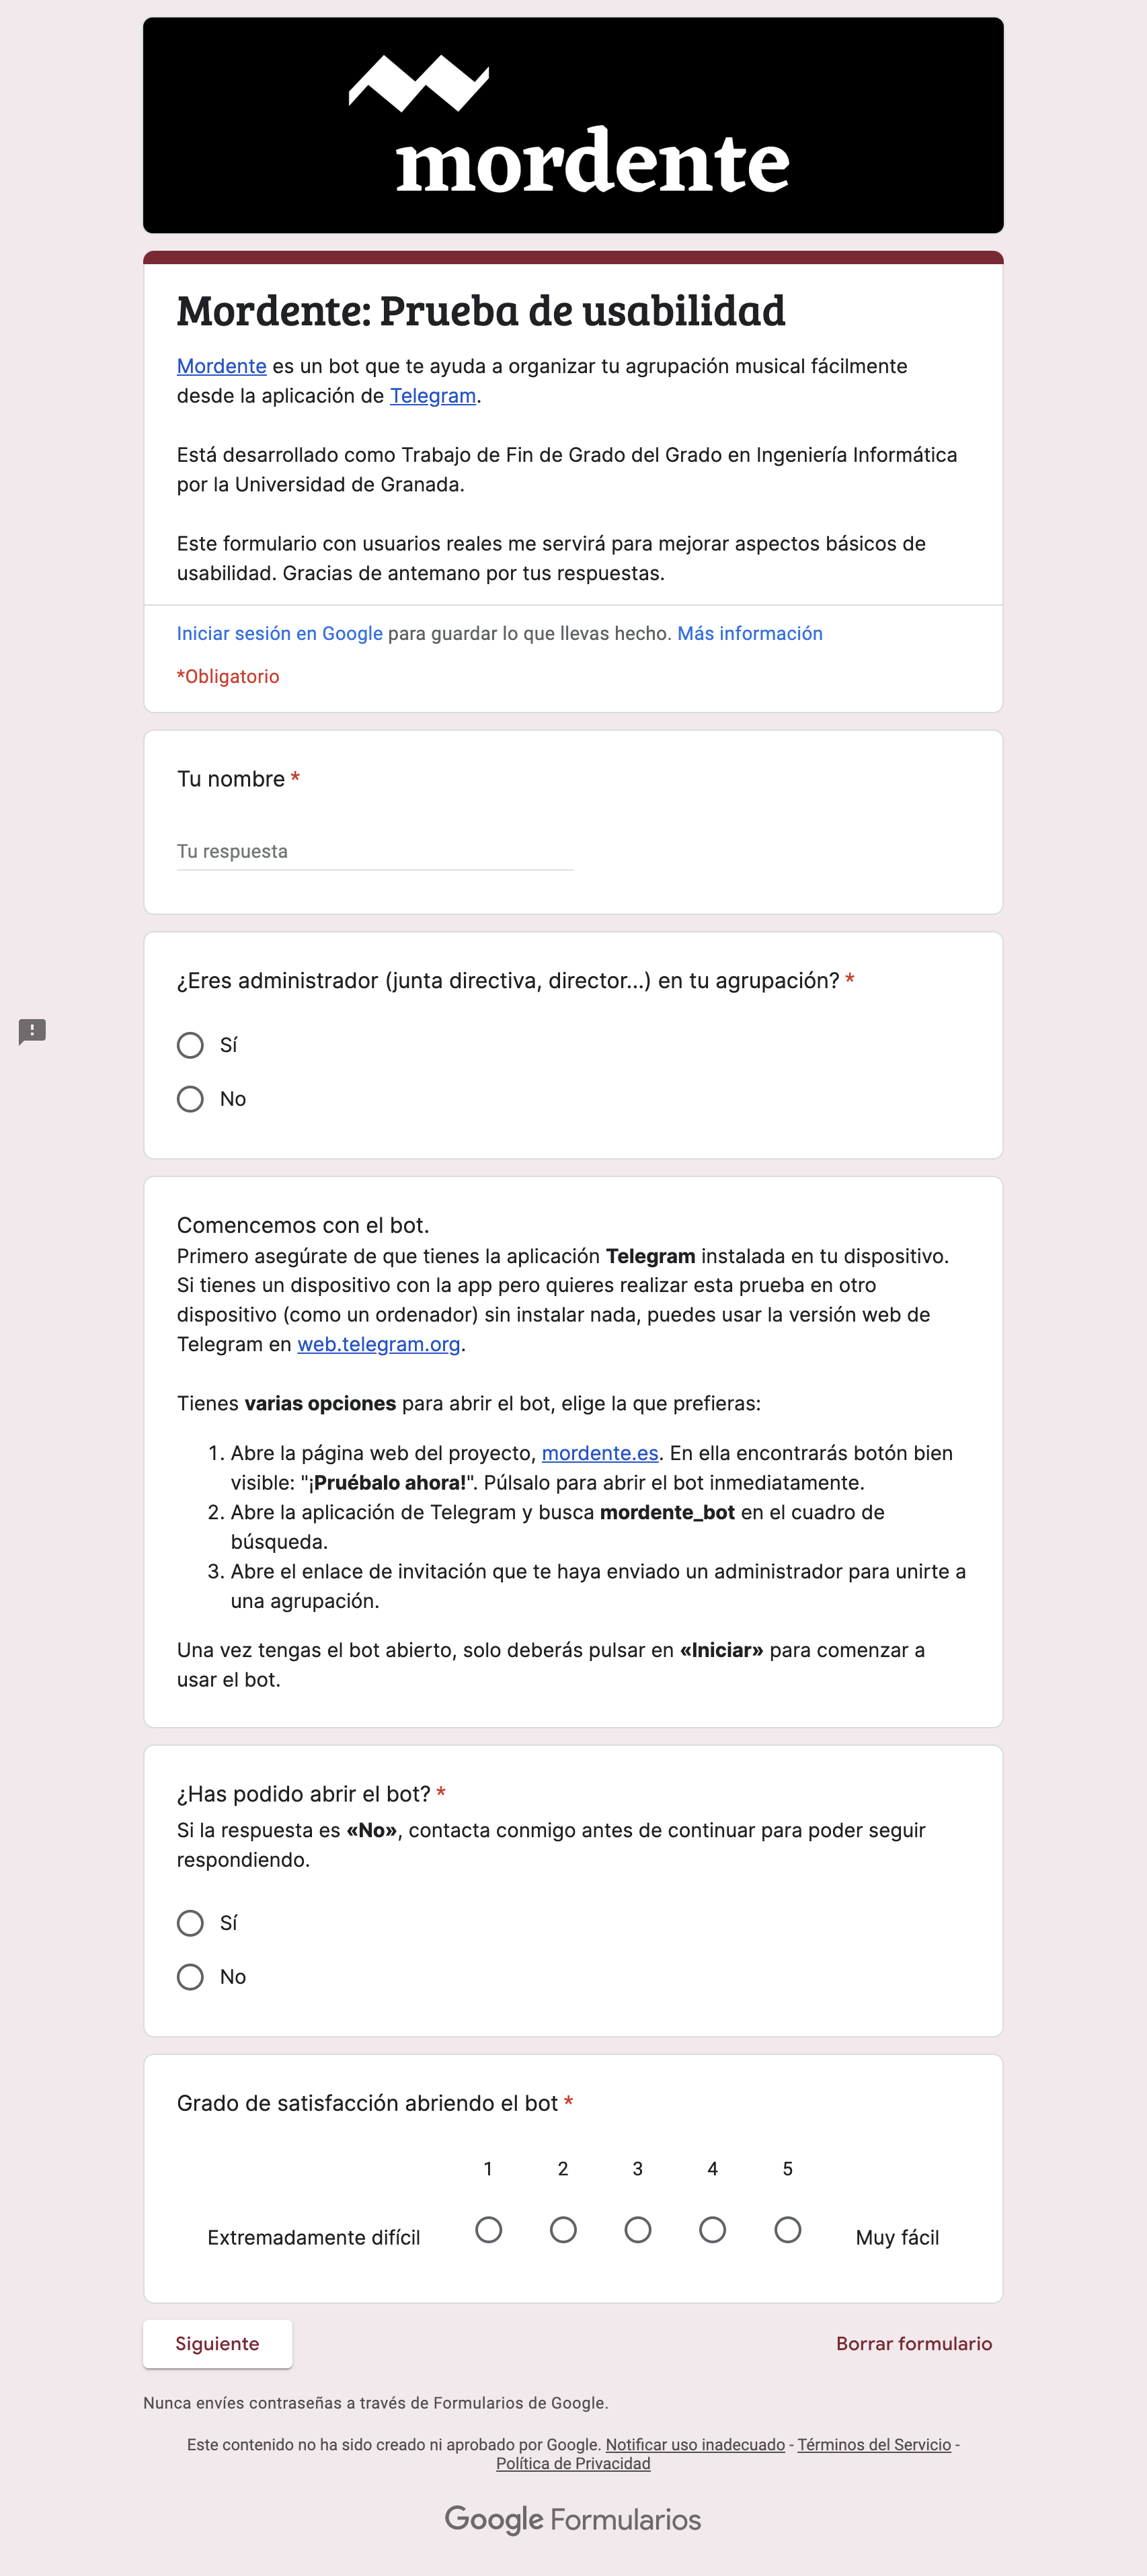
\includegraphics[width=0.65\textwidth]{imagenes/pruebas/form_1.png}
\caption{Primera página del formulario de pruebas.}
\label{fig:form1}
\end{figure}

\begin{figure}[h]
\centering
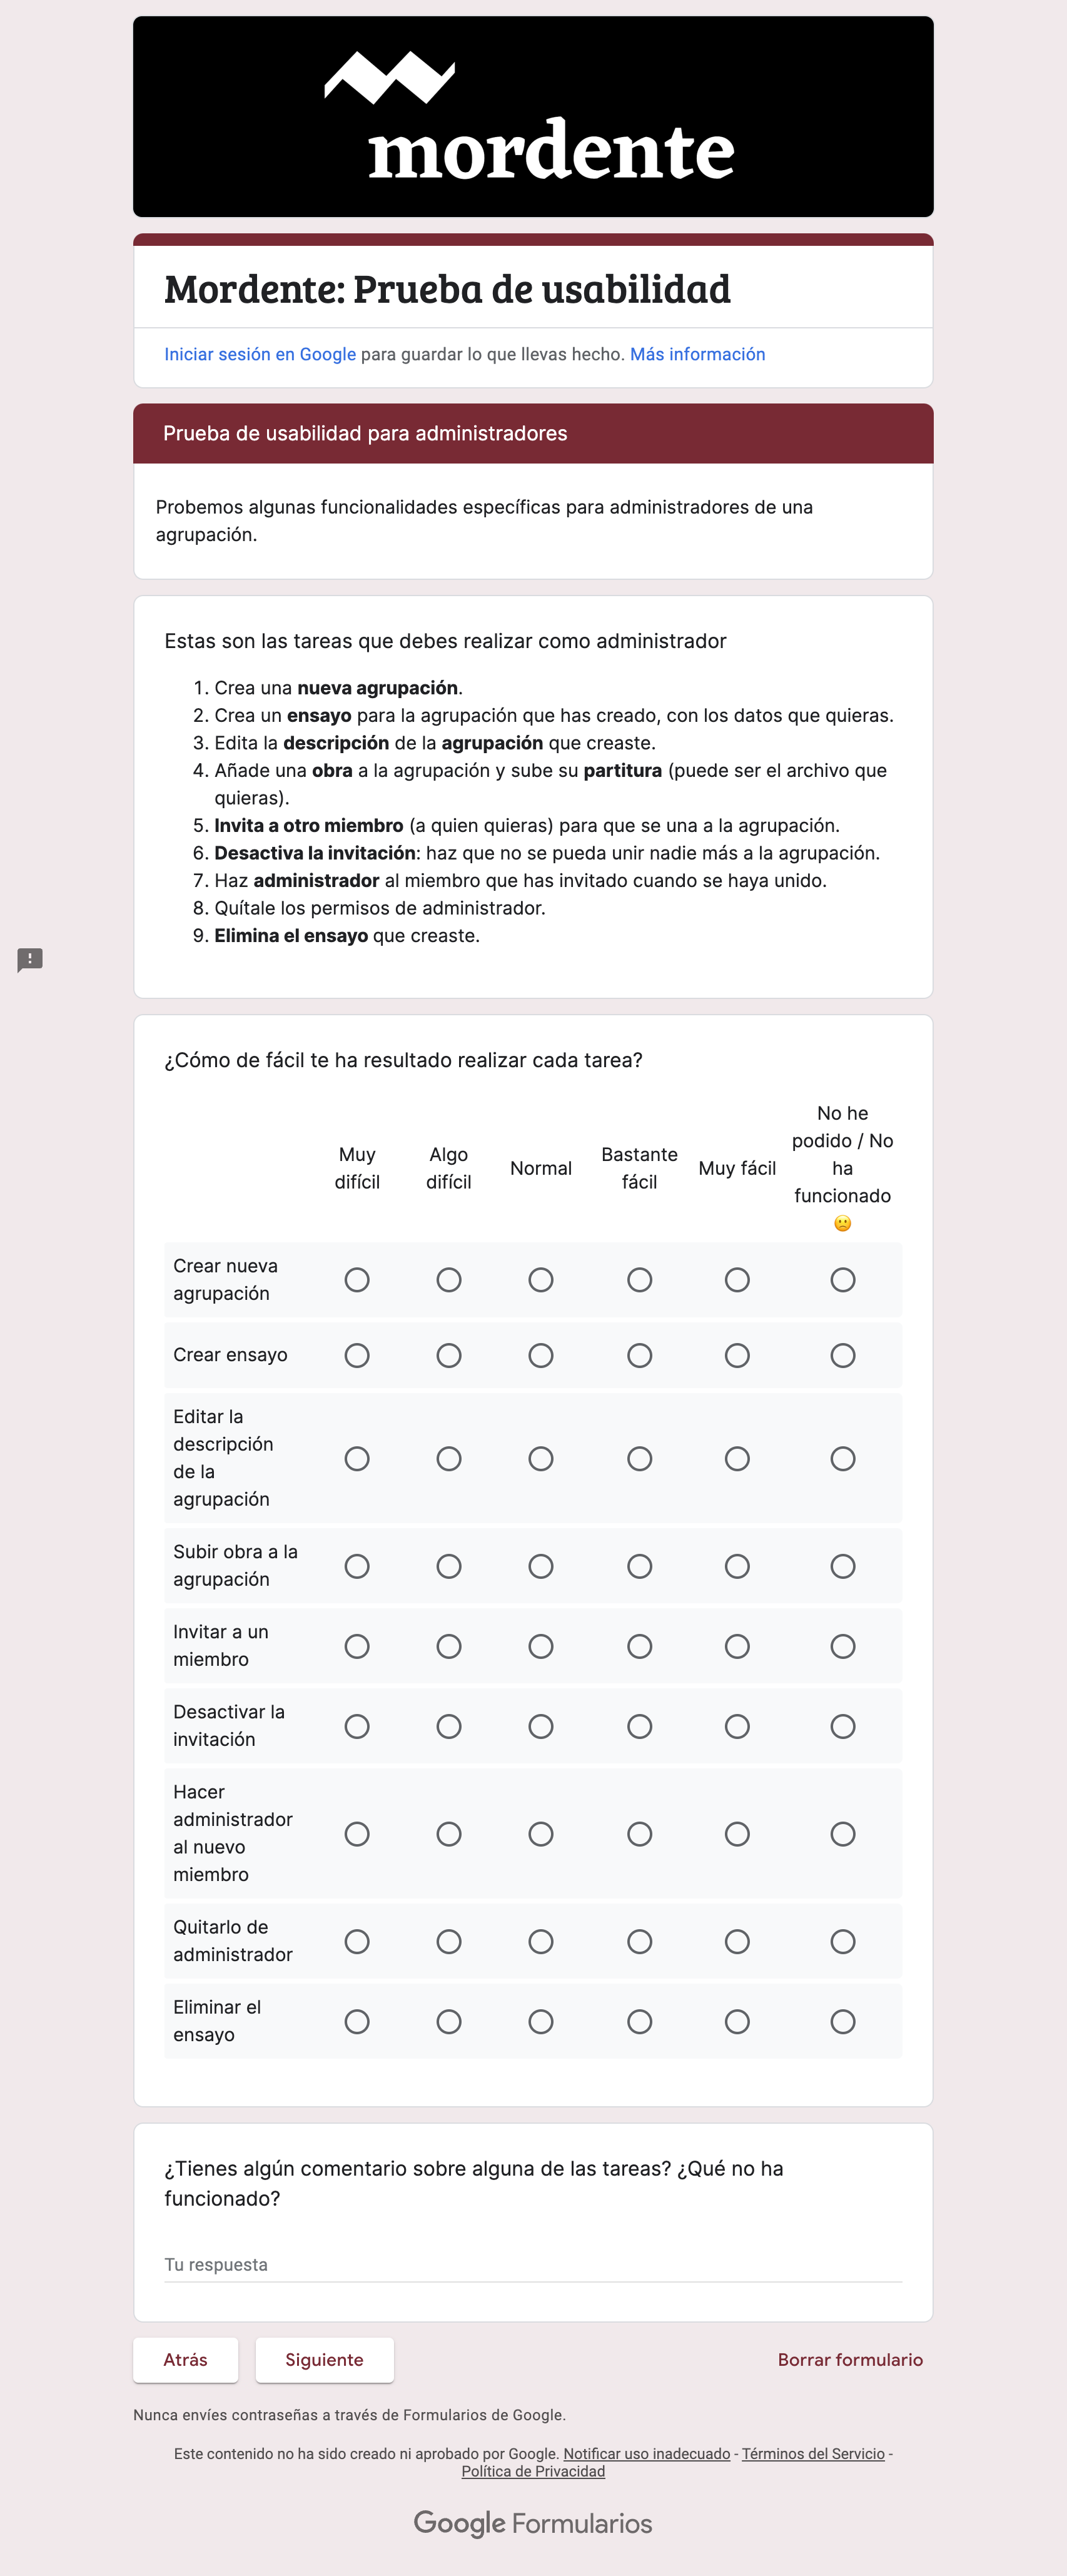
\includegraphics[width=0.6\textwidth]{imagenes/pruebas/form_2.png}
\caption{Segunda página del formulario de pruebas.}
\label{fig:form2}
\end{figure}

\begin{figure}[h]
\centering
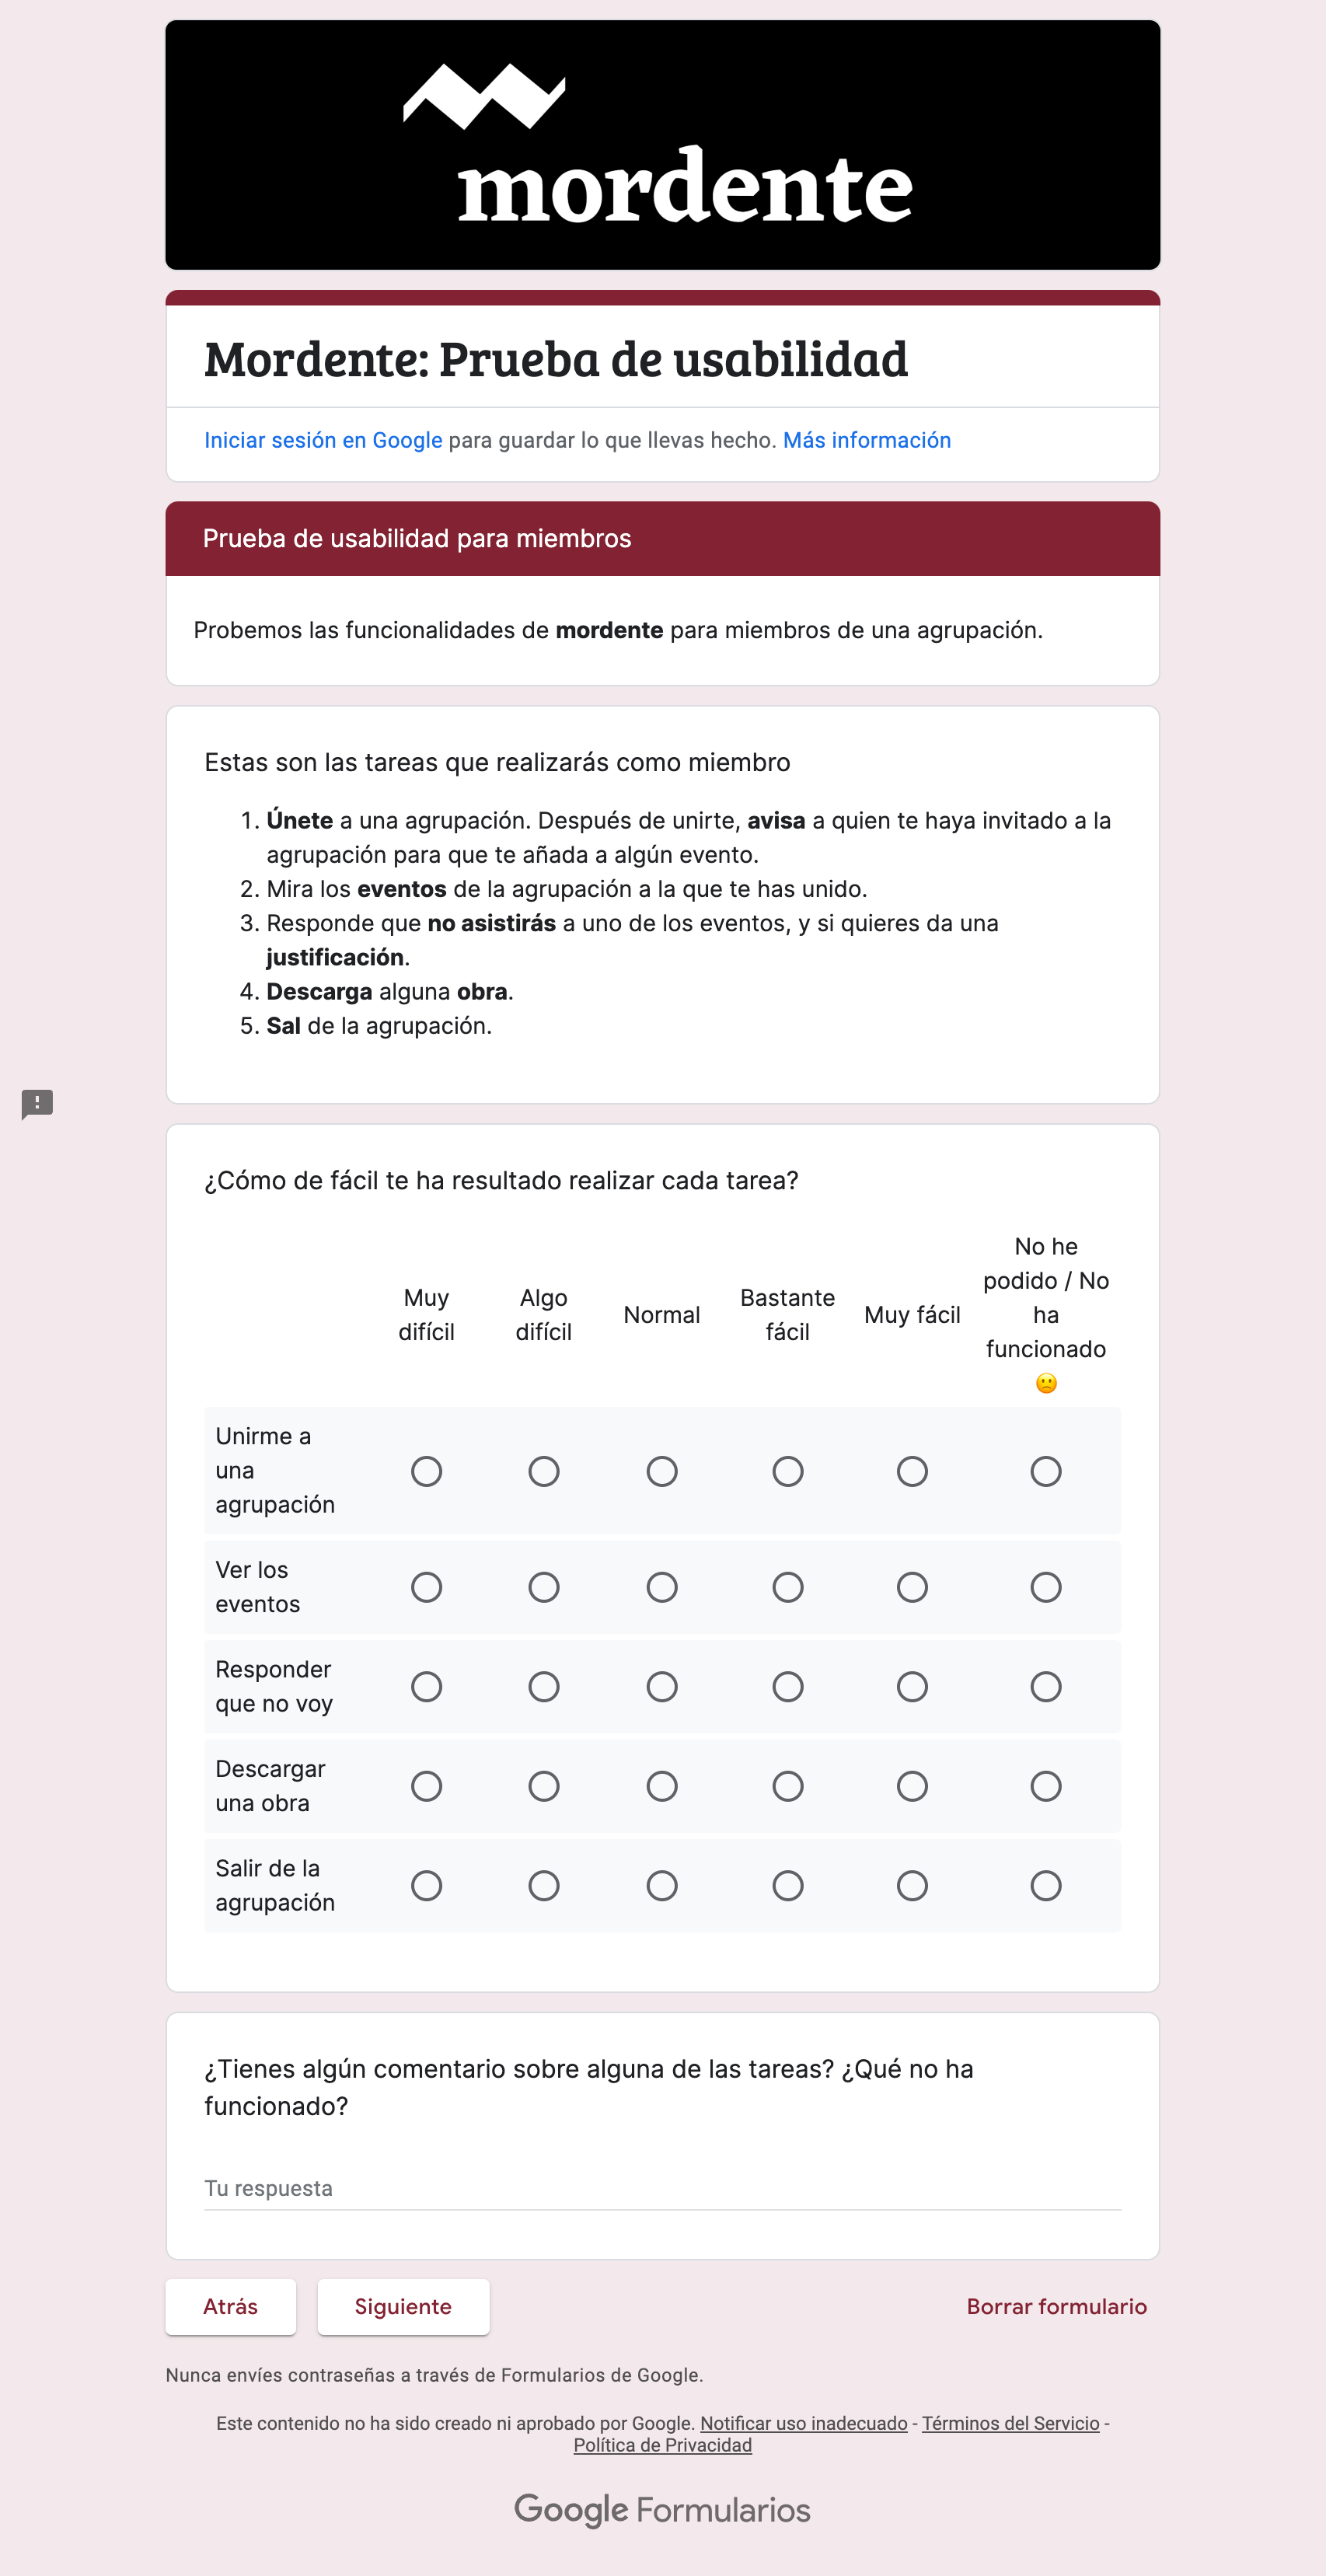
\includegraphics[width=0.75\textwidth]{imagenes/pruebas/form_3.png}
\caption{Tercera página del formulario de pruebas.}
\label{fig:form3}
\end{figure}

\begin{figure}[h]
\centering
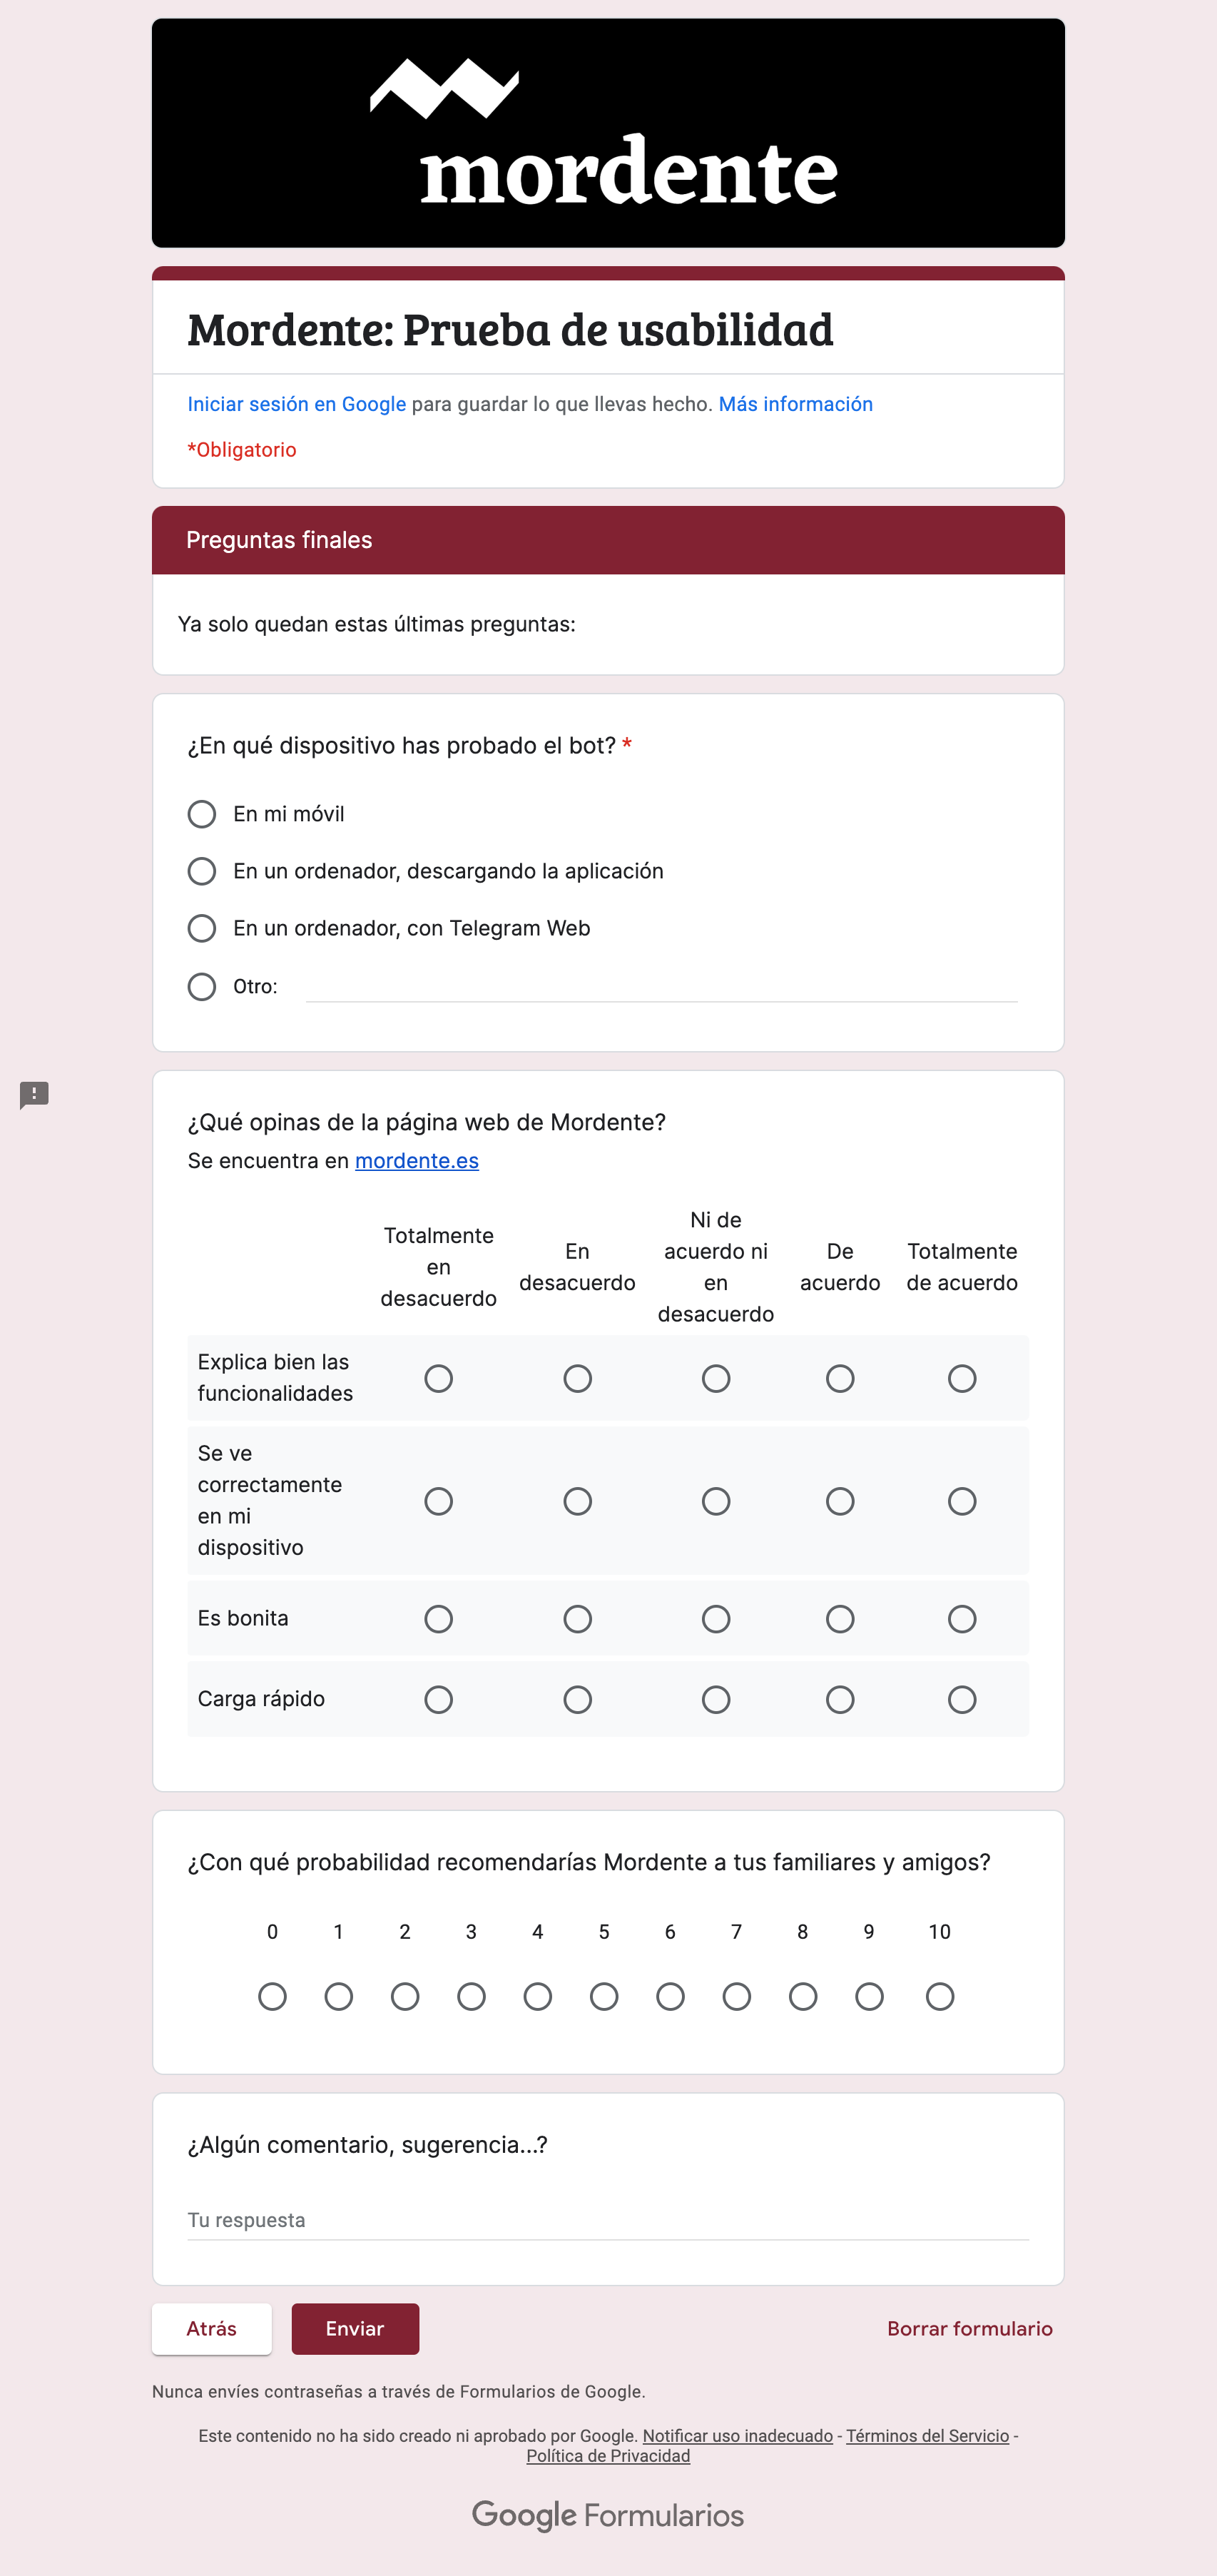
\includegraphics[width=0.7\textwidth]{imagenes/pruebas/form_4.png}
\caption{Última página del formulario de pruebas.}
\label{fig:form4}
\end{figure}

\section{Informe final de las pruebas}

\subsection{Respuestas al formulario}

Analicemos los resultados de las pruebas pregunta por pregunta:

\subsubsection{Porcentaje de administradores}

Tal y como hemos diseñado la prueba, tenemos 3 administradores y 7 miembros, por lo que el resultado es el esperado (figura \ref{fig:graficoAdministradores}).

\begin{figure}[h]
\centering
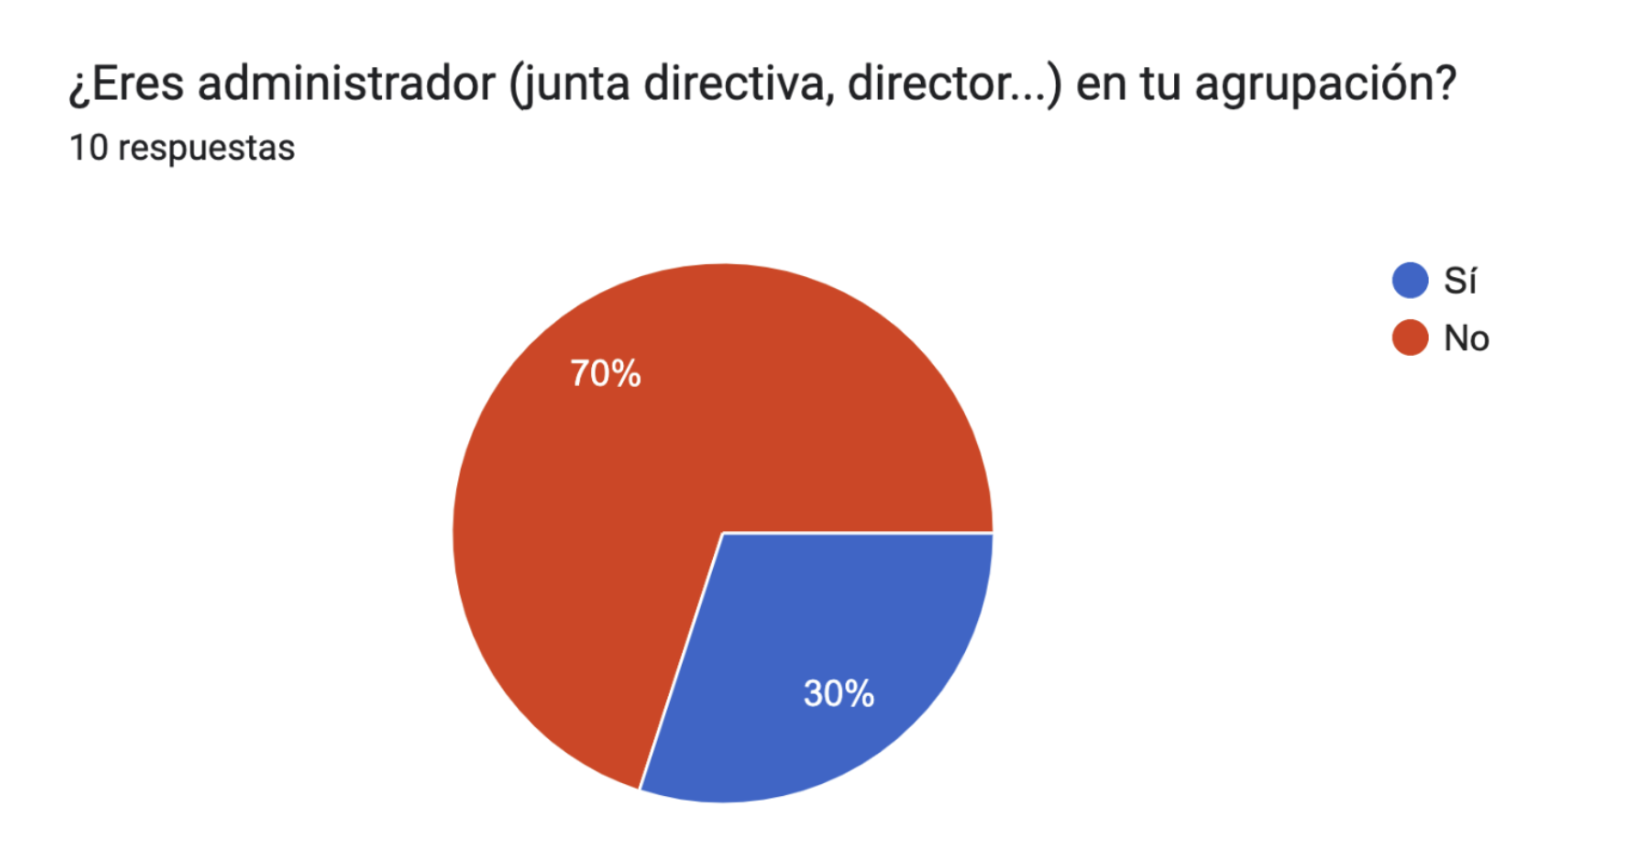
\includegraphics[width=0.75\textwidth]{imagenes/pruebas/eres_administrador.png}
\caption{Pregunta: ?`Eres administrador?}
\label{fig:graficoAdministradores}
\end{figure}

\subsubsection{?`Has podido abrir el bot?}

La respuesta de todos los usuarios ha sido positiva (figura \ref{fig:graficoAbrir}). Sin embargo, hay que aclarar que dos de los usuarios no pudieron abrir el bot hasta que se solucionaron los respectivos errores en el código, que se detallan en la sección \ref{subsection:pruebasSoluciones}.

\begin{figure}[h]
\centering
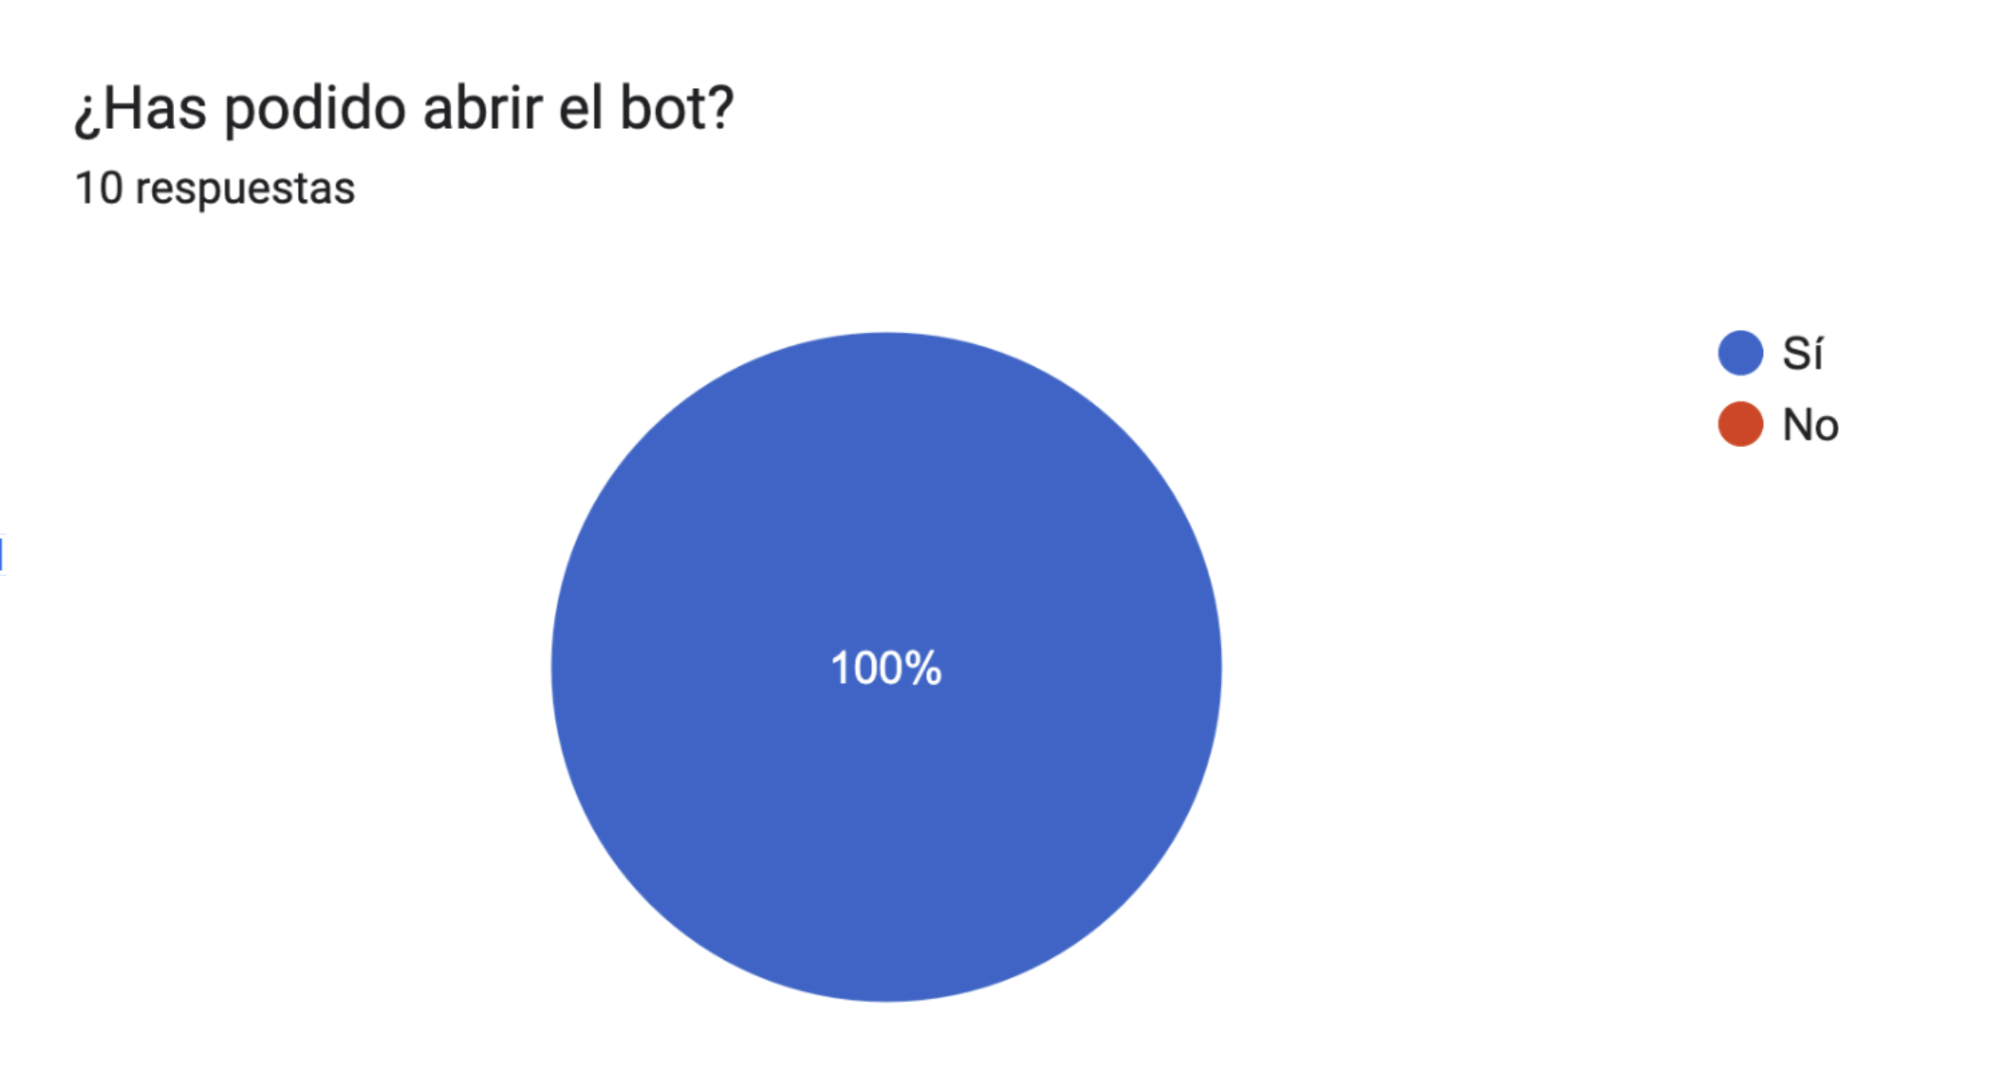
\includegraphics[width=0.75\textwidth]{imagenes/pruebas/has_podido_abrir.png}
\caption{Pregunta: ?`Has podido abrir el bot?}
\label{fig:graficoAbrir}
\end{figure}


\subsubsection{Grado de satisfacción con la apertura del bot}

En este apartado hay una respuesta unánime (figura \ref{fig:gradoSatisfaccionAbrir}): el bot es muy fácil de abrir.

Esto se debe a las múltiples opciones de acceso que hemos explicado en el formulario: especialmente desde la web \url{https://mordente.es}, que muestra un botón de apertura del bot bien visible.

\begin{figure}[h]
\centering
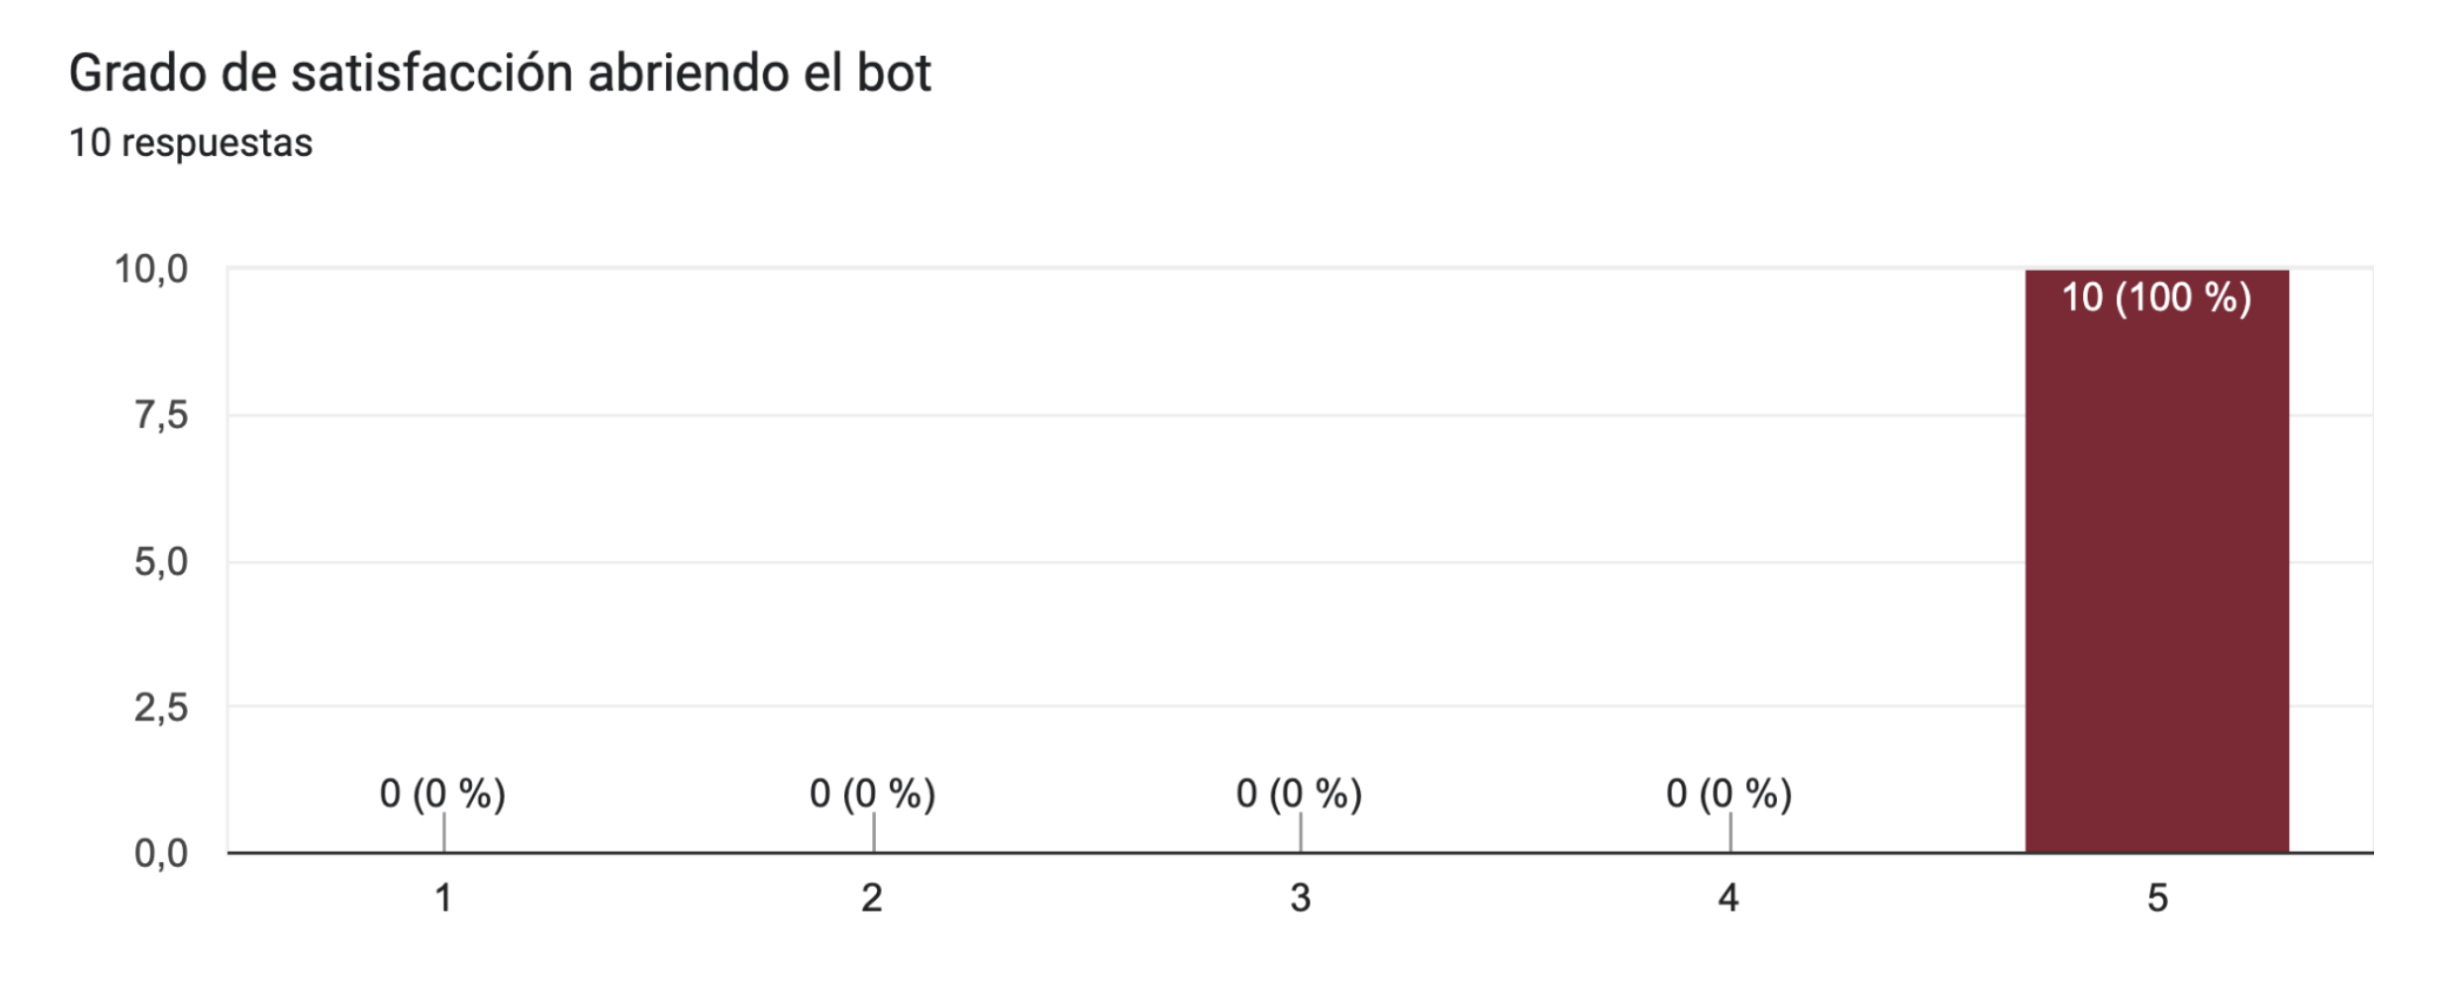
\includegraphics[width=0.9\textwidth]{imagenes/pruebas/grado_satisfaccion_abriendo.png}
\caption{Grado de satisfacción abriendo el bot.}
\label{fig:gradoSatisfaccionAbrir}
\end{figure}

\subsubsection{Tareas de administrador}

Los resultados de las preguntas se pueden ver en la figura \ref{fig:graficoTareasAdmin}. A continuación vamos a comentar las posibles mejoras y las causas de las respuestas positivas:

\begin{itemize}
    \item \textbf{Crear nueva agrupación:} Muy fácil para todos los encuestados. El bot muestra un botón para crear una agrupación justo al abrirlo por primera vez.
    \item \textbf{Crear ensayo:} 2 usuarios responden ``bastante fácil'' y 1 ``muy fácil''. La usabilidad es menor por tener que acceder a la lista de eventos para crearlo. Se puede considerar añadir el botón de \texttt{Crear evento} en el detalle de una agrupación.
    \item \textbf{Editar la descripción de una agrupación:} todos los usuarios responden ``muy fácil''. El botón de editar se encuentra directamente en el detalle de la agrupación y solo se edita un campo, por lo que es rápido.
    \item \textbf{Subir obra a la agrupación:} 2 usuarios responden ``muy fácil'' y 1 ``bastante fácil''. La mejora posible sería hacer que se puedan subir obras sin acceder al menú de una agrupación.
    \item \textbf{Invitar a un miembro:} Las respuestas son de un peor resultado. Uno de los comentarios nos advierte de la razón: no se está explicando qué se debe hacer con el enlace de invitación. Añadiremos un mensaje explicativo de su función.
    \item \textbf{Desactivar la invitación:} todas las respuestas son buenas, de modo que el botón para desactivar la invitación se entiende claramente.
    \item \textbf{Hacer administrador al nuevo miembro:} La mayoría de respuestas son muy positivas.
    \item \textbf{Quitar los permisos de administrador al nuevo miembro:} Mismas respuestas de la pregunta anterior.
    \item \textbf{Eliminar el ensayo creado:} Dos respuestas muy positivas y una positiva. Es un buen resultado teniendo en cuenta que se pide una confirmación.
\end{itemize}

\begin{figure}[h]
\centering
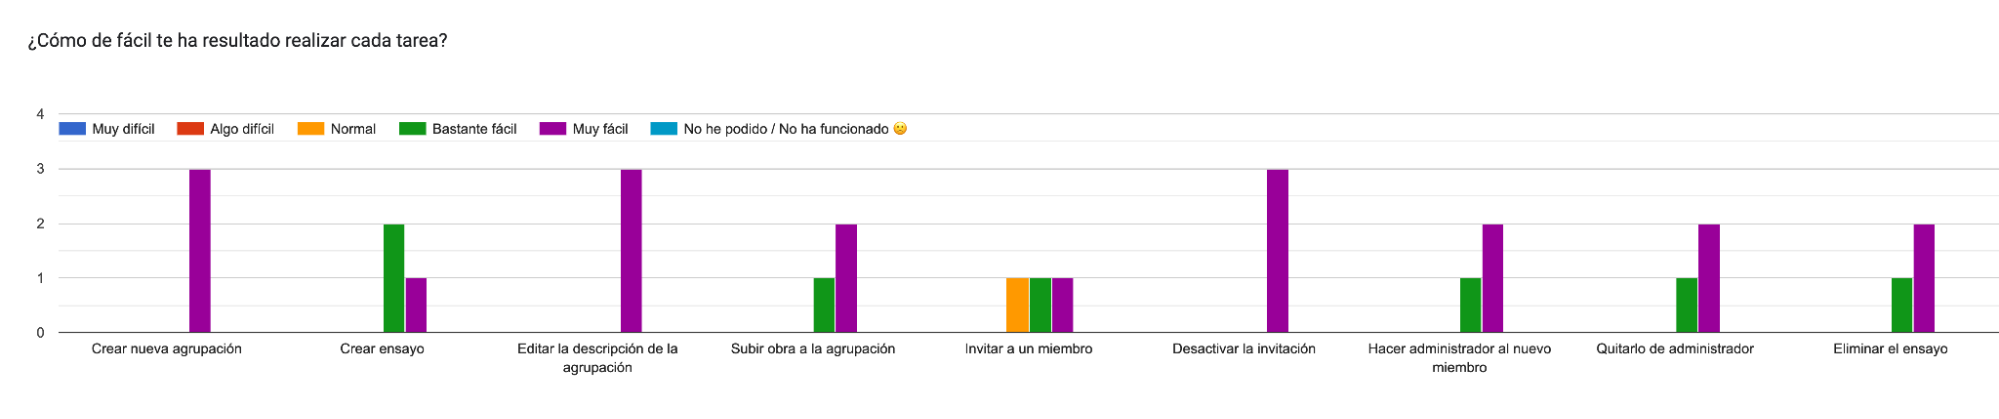
\includegraphics[width=\textwidth]{imagenes/pruebas/tareas_admin.png}
\caption{Grado de dificultad de las tareas de administrador.}
\label{fig:graficoTareasAdmin}
\end{figure}

\subsubsection{Tareas de miembro}

Al igual que las tareas de administrador, los resultados de las preguntas se pueden ver en la figura \ref{fig:graficoTareasMiembro}. Hagamos algunos comentarios:

\begin{itemize}
    \item \textbf{Unirme a una agrupación:} Casi todos los usuarios manifiestan que es ``muy fácil''. El enlace de invitación hace que los usuarios solo tengan que abrirlo para unirse.
    \item \textbf{Ver los eventos:} Como se manifiesta en uno de los comentarios, deberíamos hacer más visible la función de \textbf{resumen de eventos}. Esto también va relacionado con la petición de \textbf{función de calendario}.
    \item \textbf{Responder que no voy:} Los usuarios consideran mayoritariamente que es muy fácil porque se puede responder directamente desde el menú de un evento.
    \item \textbf{Descargar una obra:} Las obras se pueden pedir directamente desde el menú de una agrupación, después solo hay que pulsar en \texttt{Descargar}. Todos los usuarios lo hallan muy fácil.
    \item \textbf{Salir de una agrupación:} Los resultados son menos óptimos, y hay un comentario sobre esto. Podríamos añadir la opción al menú de agrupación para no tener que abrir el de membresía.
\end{itemize}

\begin{figure}[h]
\centering
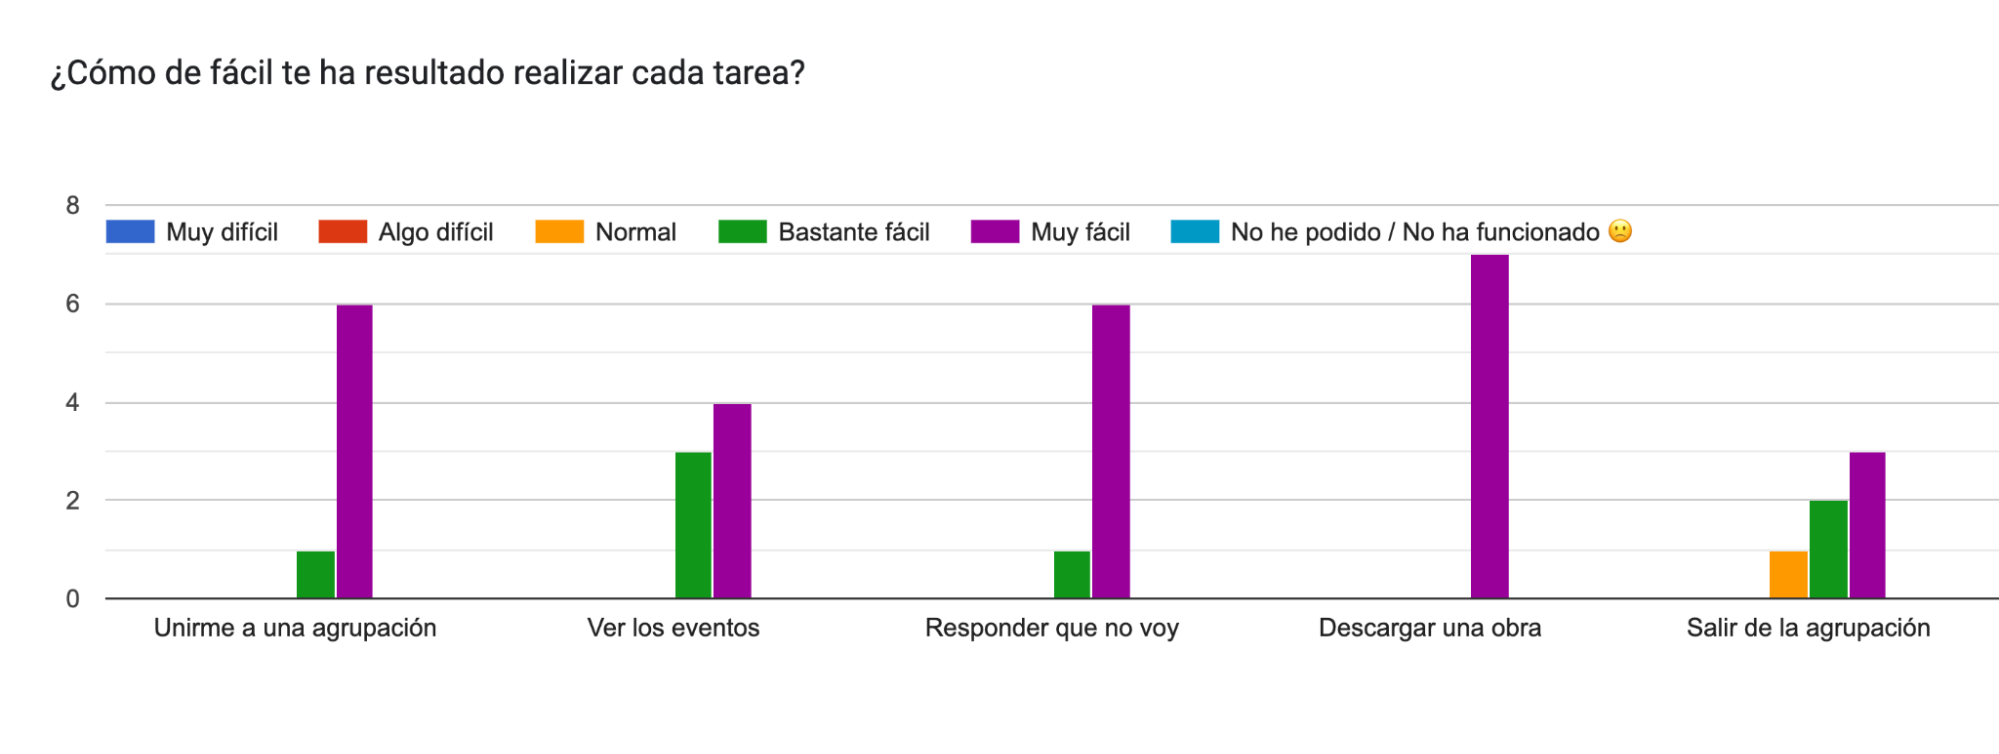
\includegraphics[width=\textwidth]{imagenes/pruebas/tareas_miembro.png}
\caption{Grado de dificultad de las tareas de miembro.}
\label{fig:graficoTareasMiembro}
\end{figure}

En este apartado se han recibido varios comentarios, mostrados en la tabla \ref{tab:comentariosTareasMiembro}. Todos ellos tienen un contenido interesante:
\begin{itemize}
    \item Destaca la petición común de la \textbf{función de calendario}, que vemos a lo largo de las pruebas.
    \item Un usuario manifiesta que tiene que dar demasiados pasos para \textbf{ver los eventos}. Quizás deberíamos reforzar la visibilidad de la función de \textbf{resumen de eventos}.
    \item \textbf{Unirse al bot} le genera dudas a un usuario, ya que siempre aparece el botón \texttt{INICIAR} aunque ya se haya iniciado el bot. Esto podría explicarse en el mensaje que incluye el enlace de invitación.
    \item La función de \textbf{salir de una agrupación} está en el menú de la membresía. Se podría añadir también al menú del detalle de un evento para una mayor visibilidad.
\end{itemize}

\begin{table}[h!]
\centering
\begin{tabularx}{\textwidth}{|X|} 
\hline
Podría haber un calendario para ver los eventos, pero por lo demás funciona muy bien. \\
\hline
Demasiados pasos para ver los eventos. \\
\hline
No sabía qué hacer para unirme a la agrupación si ya había iniciado el bot \\
\hline
No encontraba la opción de salir de la agrupación \\
\hline
\end{tabularx}
\caption{Comentarios a las tareas de miembro de las pruebas.}
\label{tab:comentariosTareasMiembro}
\end{table}

\subsubsection{Dispositivo de pruebas}

El 80\% de los encuestados han hecho las pruebas desde móvil, y el 20\% desde la aplicación de escritorio, como podemos ver en la figura \ref{fig:graficoDispositivo}. La responsabilidad de hacer que el bot funcione en todos los dispositivos está delegada a Telegram, por lo que no encontramos ningún problema en ese aspecto.

\begin{figure}[h]
\centering
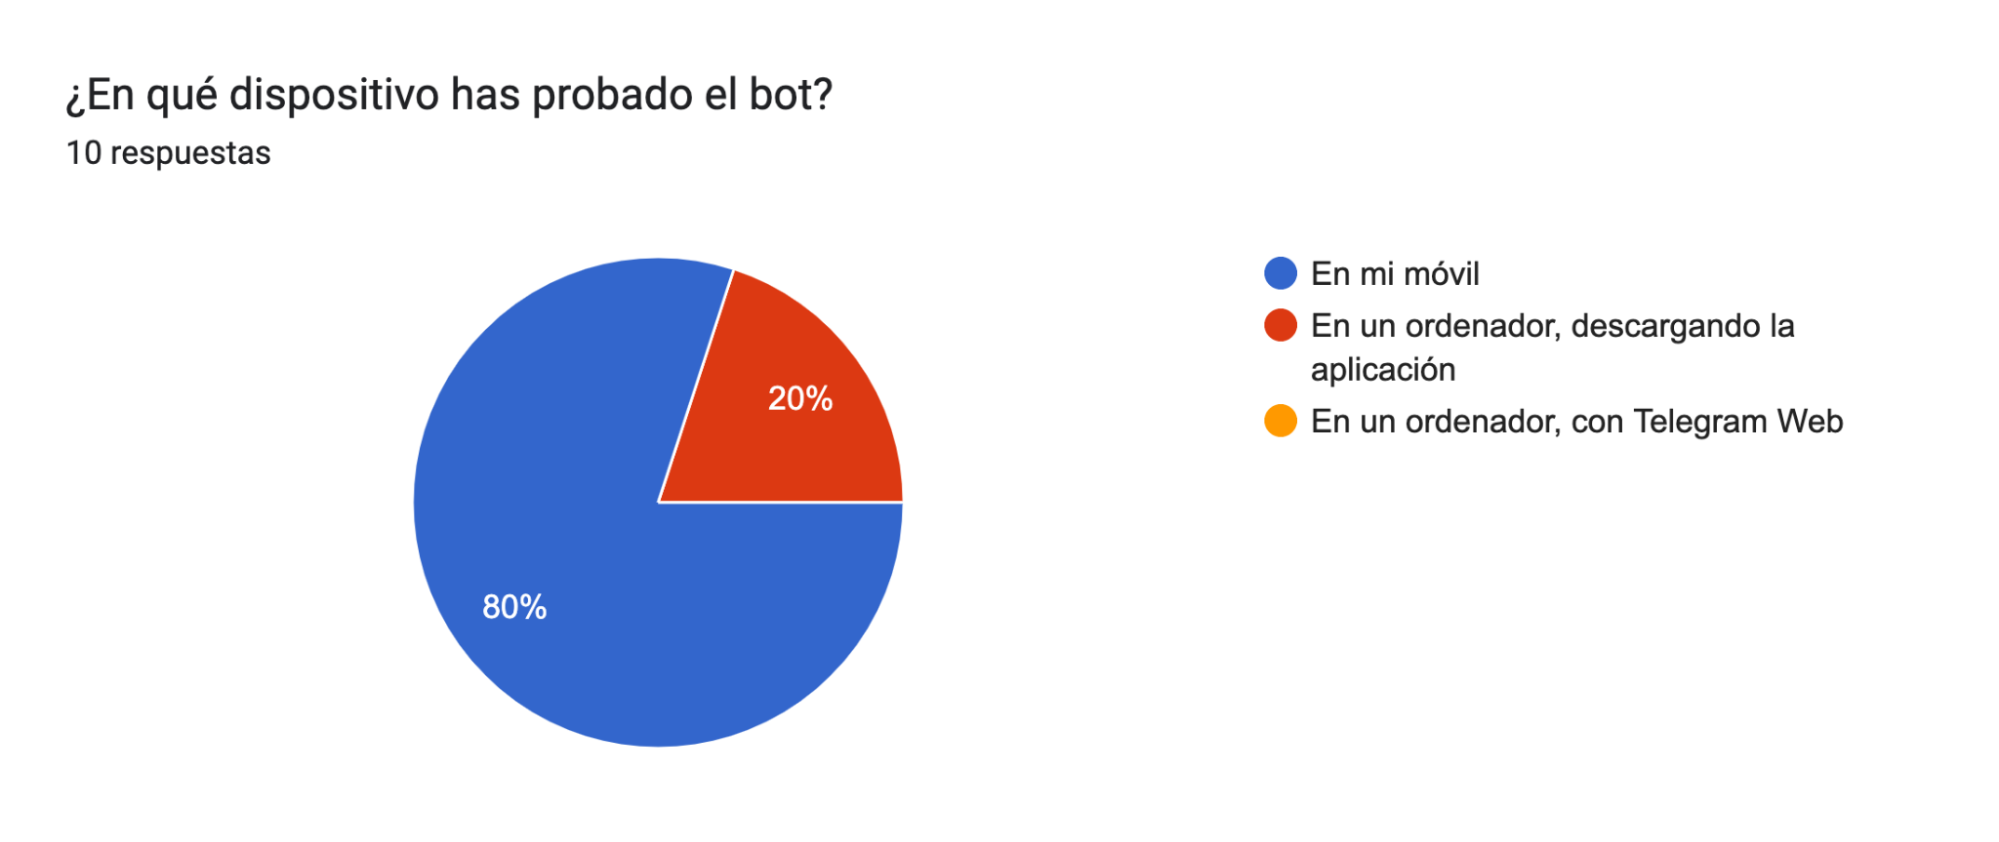
\includegraphics[width=\textwidth]{imagenes/pruebas/dispositivo.png}
\caption{Dispositivo utilizado para las pruebas.}
\label{fig:graficoDispositivo}
\end{figure}

\subsubsection{Página web}

Comentemos los resultados de la figura \ref{fig:satisfaccionWeb}:

\begin{itemize}
    \item \textbf{Buena explicación de funcionalidades:} Es la pregunta con peores resultados. Se entiende que hay que mejorar el tutorial e incluir explicaciones más completas y sobre más funcionalidades del bot.
    \item \textbf{Buen diseño para distintos dispositivos:} Todas las respuestas son muy buenas. Esto demuestra que usar \texttt{docusaurus} para construir la página web ha sido una buena elección.
    \item \textbf{Buena apariencia:} Casi todas las respuestas son muy buenas. La posible actuación sería mejorar los colores del tema oscuro.
    \item \textbf{Carga rápida:} Todos los encuestados están totalmente de acuerdo en que la web carga rápido. La página web se sirve en caché desde París, por lo que queda demostrado que la elección de proveedor ha sido correcta.
\end{itemize}

\begin{figure}[h]
\centering
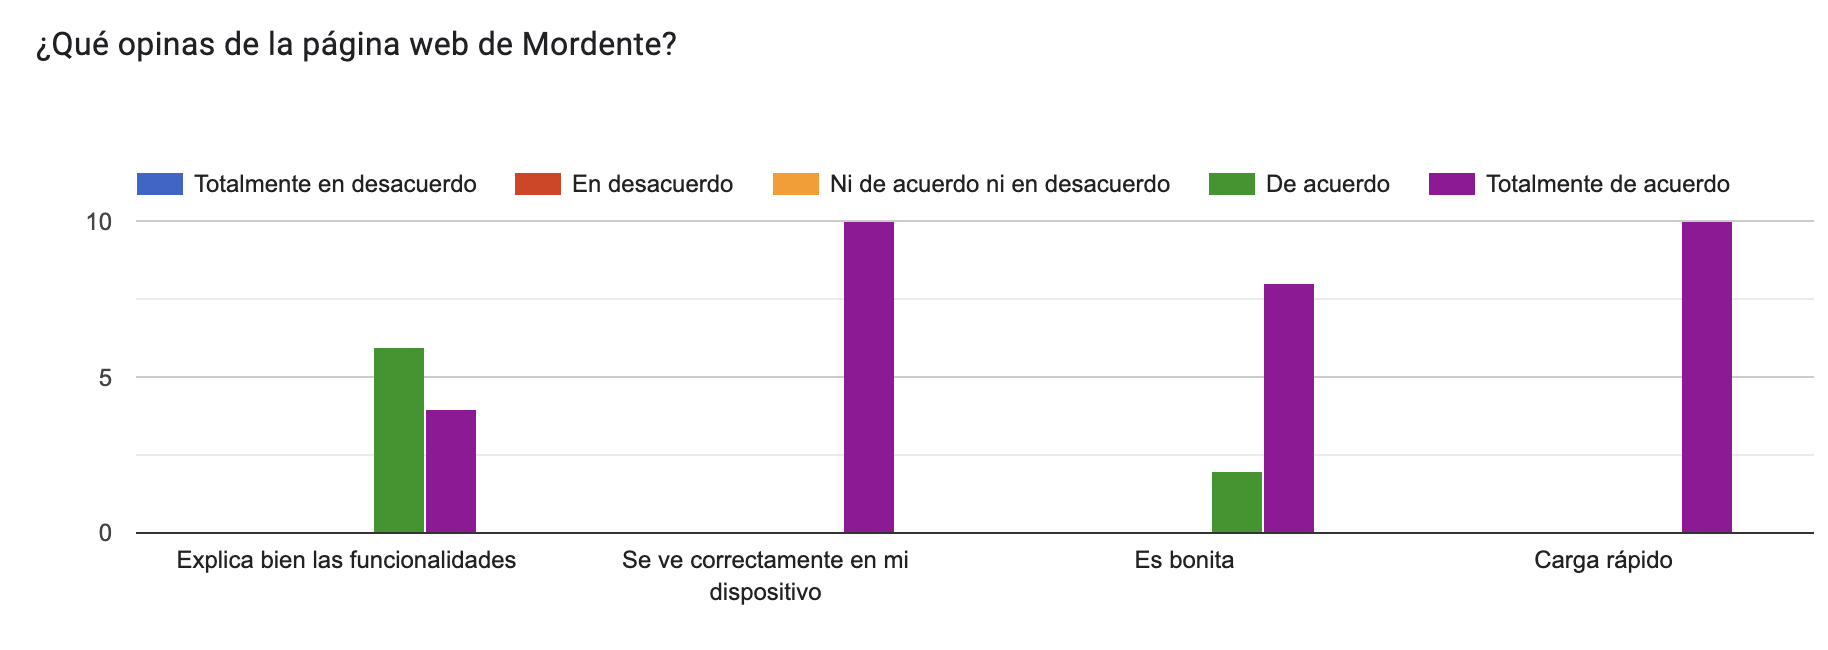
\includegraphics[width=\textwidth]{imagenes/pruebas/web.png}
\caption{Grado de satisfacción con la página web.}
\label{fig:satisfaccionWeb}
\end{figure}

\subsubsection{NET Promoter Score (NPS)}

Las respuestas a esta pregunta están representadas en la figura \ref{fig:graficoNetScore}.
Para calcular el \textbf{Net Promoter Score} vamos a seguir la fórmula:

\begin{equation*}
\begin{aligned}
\textrm{NPS} ={} & \frac{\textrm{Promotores} - \textrm{Detractores}}{\textrm{Encuestados}} \times 100 \\
={} & \frac{9-1}{10} \times 100 = 80
\end{aligned}
\end{equation*}

El valor resultante es 80, lo cual entra dentro del rango \textbf{excelente} por ser superior a 50.

\begin{figure}[h]
\centering
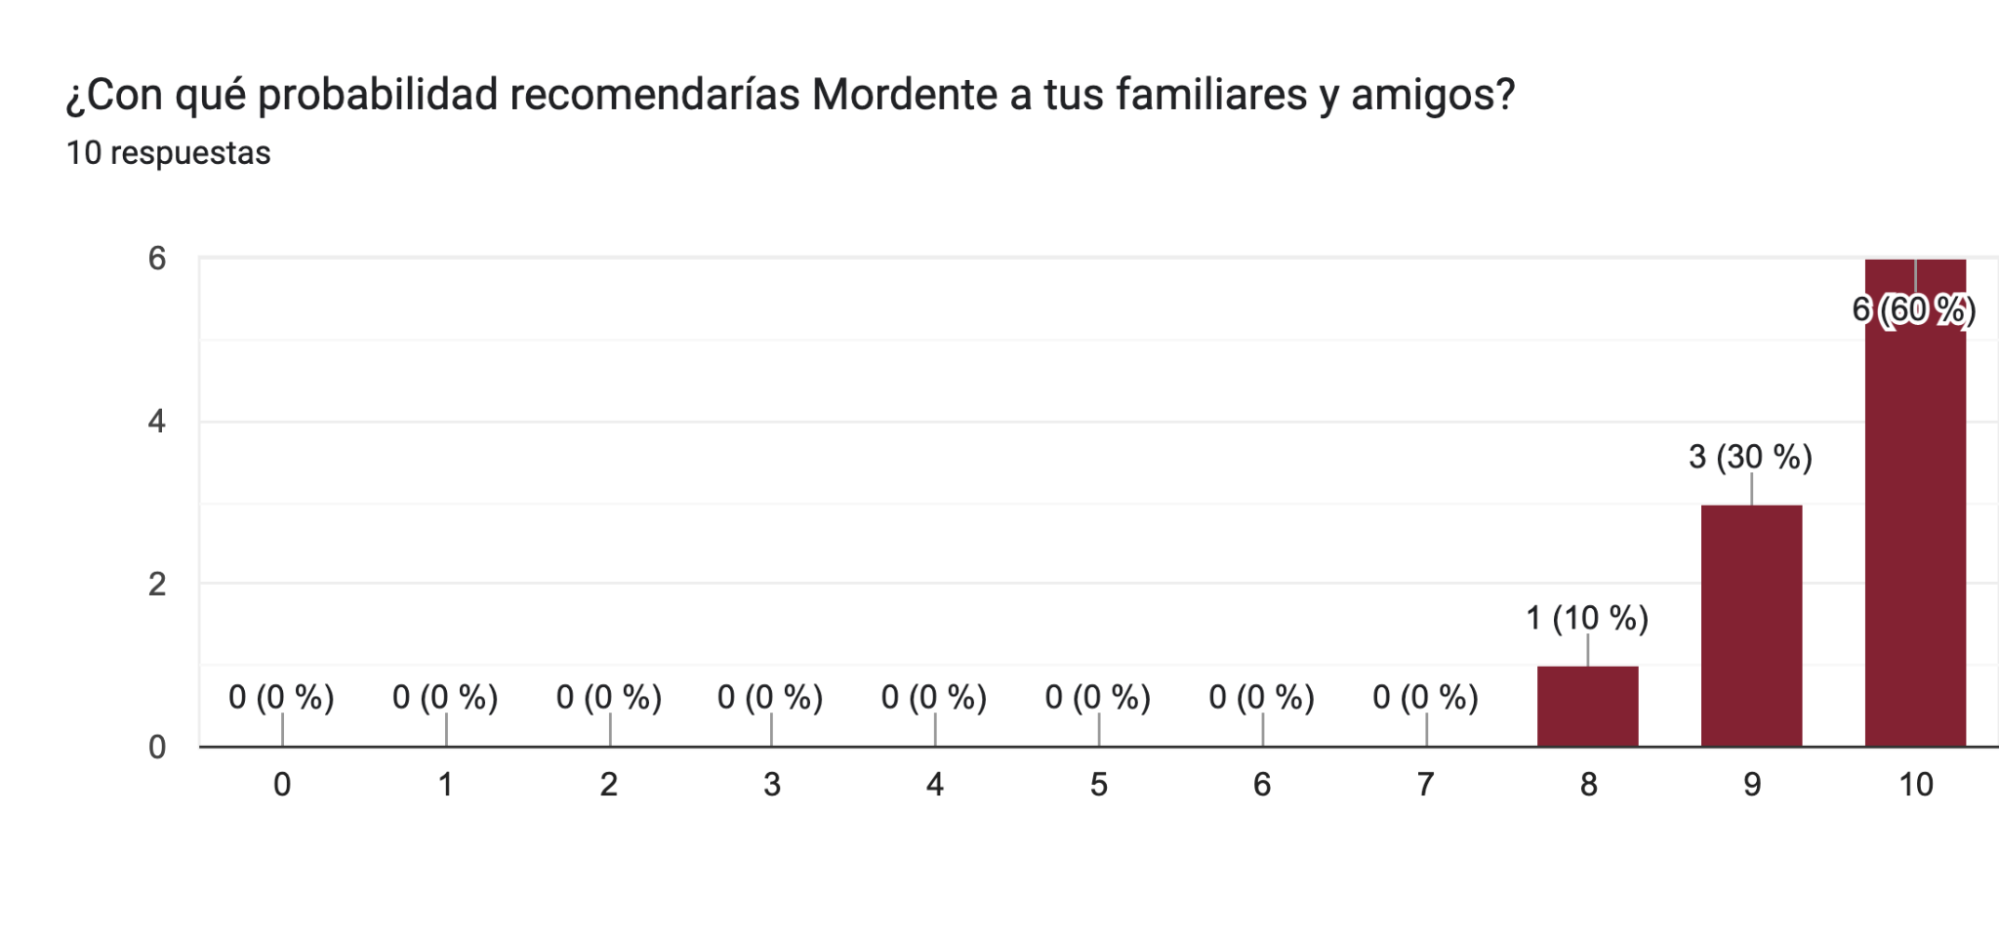
\includegraphics[width=\textwidth]{imagenes/pruebas/recomendacion.png}
\caption{Pregunta: ?`Recomendarías \textbf{Mordente} a tus familiares y amigos?}
\label{fig:graficoNetScore}
\end{figure}

\subsubsection{Comentarios generales}

Se han recibido cuatro comentarios, expuestos en la tabla \ref{tab:respuestasComentarios}.

\begin{table}[h!]
\centering
\begin{tabularx}{\textwidth}{|X|} 
 \hline
 Al principio no funcionaba el bot. Me he puesto en contacto para solucionarlo y ya sí he podido. \\ 
 \hline
 Muy intuitivo e inmediato \\
 \hline
 Añadir calendario, añadir diseño de escenario, poder extraer gráficas de asistencia \\
 \hline
 \makecell[l]{No podía abrir el bot al principio, pero se ha solucionado. \\ Estaría bien ver los eventos en un calendario.} \\
 \hline
\end{tabularx}
\caption{Comentarios generales al formulario de pruebas.}
\label{tab:respuestasComentarios}
\end{table}

De estos comentarios se extrae la petición popular de añadir la función de calendario, y se deja constancia del problema que han manifestado dos usuarios que no pudieron abrir el bot por encontrarse con un error. Estos errores se resolverán en la sección \ref{subsection:pruebasSoluciones}.

El director de la agrupación donde se han hecho las pruebas sugiere añadir las funciones de crear un diseño del escenario y gráficas de asistencia. El diseño del escenario requiere una aplicación web, por lo que se incluirá dentro de ese futuro proyecto.

\subsection{Problemas detectados y su solución}\label{subsection:pruebasSoluciones}

A continuación se relatan los problemas más graves encontrados durante la realización de las pruebas, y que impedían a algunos usuarios comenzar a usar el bot.

\subsubsection{Campo \texttt{username} vacío en algunos usuarios}

Uno de los problemas detectados durante las pruebas viene derivado por el hecho de que Telegram no obliga a los usuarios a asignarse un nombre de usuario, por lo que el campo \texttt{username} de nuestra base de datos se queda vacío. Esto resultaba en una excepción controlada a la hora de actualizar sus datos que se ha corregido\footnote{\url{https://github.com/daniharo/mordente/commit/70b3b54}}.

\subsubsection{Desbordamiento del campo de ID de Telegram}

Uno de los usuarios que realizaron las pruebas se puso en contacto para manifestar que no era capaz de obtener ninguna respuesta por parte del bot: siempre obtenía un mensaje de error.

Revisando \textbf{Sentry} (sección \ref{subsection:sentry}), vemos que se ha registrado el error (figuras \ref{fig:sentryListaErrores} y \ref{fig:sentryDetalleError}) y que se debe a que el ID de Telegram del usuario no cabe en el tipo \texttt{INTEGER} de \textbf{PostgreSQL}. Revisando la documentación de Telegram\footnote{\url{https://core.telegram.org/bots/api\#chat}}, descubrimos efectivamente que los IDs de Telegram pueden ocupar hasta 52 bits, mientras el tipo \texttt{INTEGER} alberga hasta 32 bits incluyendo el signo.

Para solucionar el problema, migramos la columna \texttt{uid} de la tabla \texttt{User} al tipo \texttt{Float} de Prisma aplicando la correspondiente migración de la base de datos\footnote{\textit{Commit:} \url{https://github.com/daniharo/mordente/commit/46f665c0}}, de forma que el usuario ya pudo terminar las pruebas correctamente.

\begin{figure}[h]
\centering
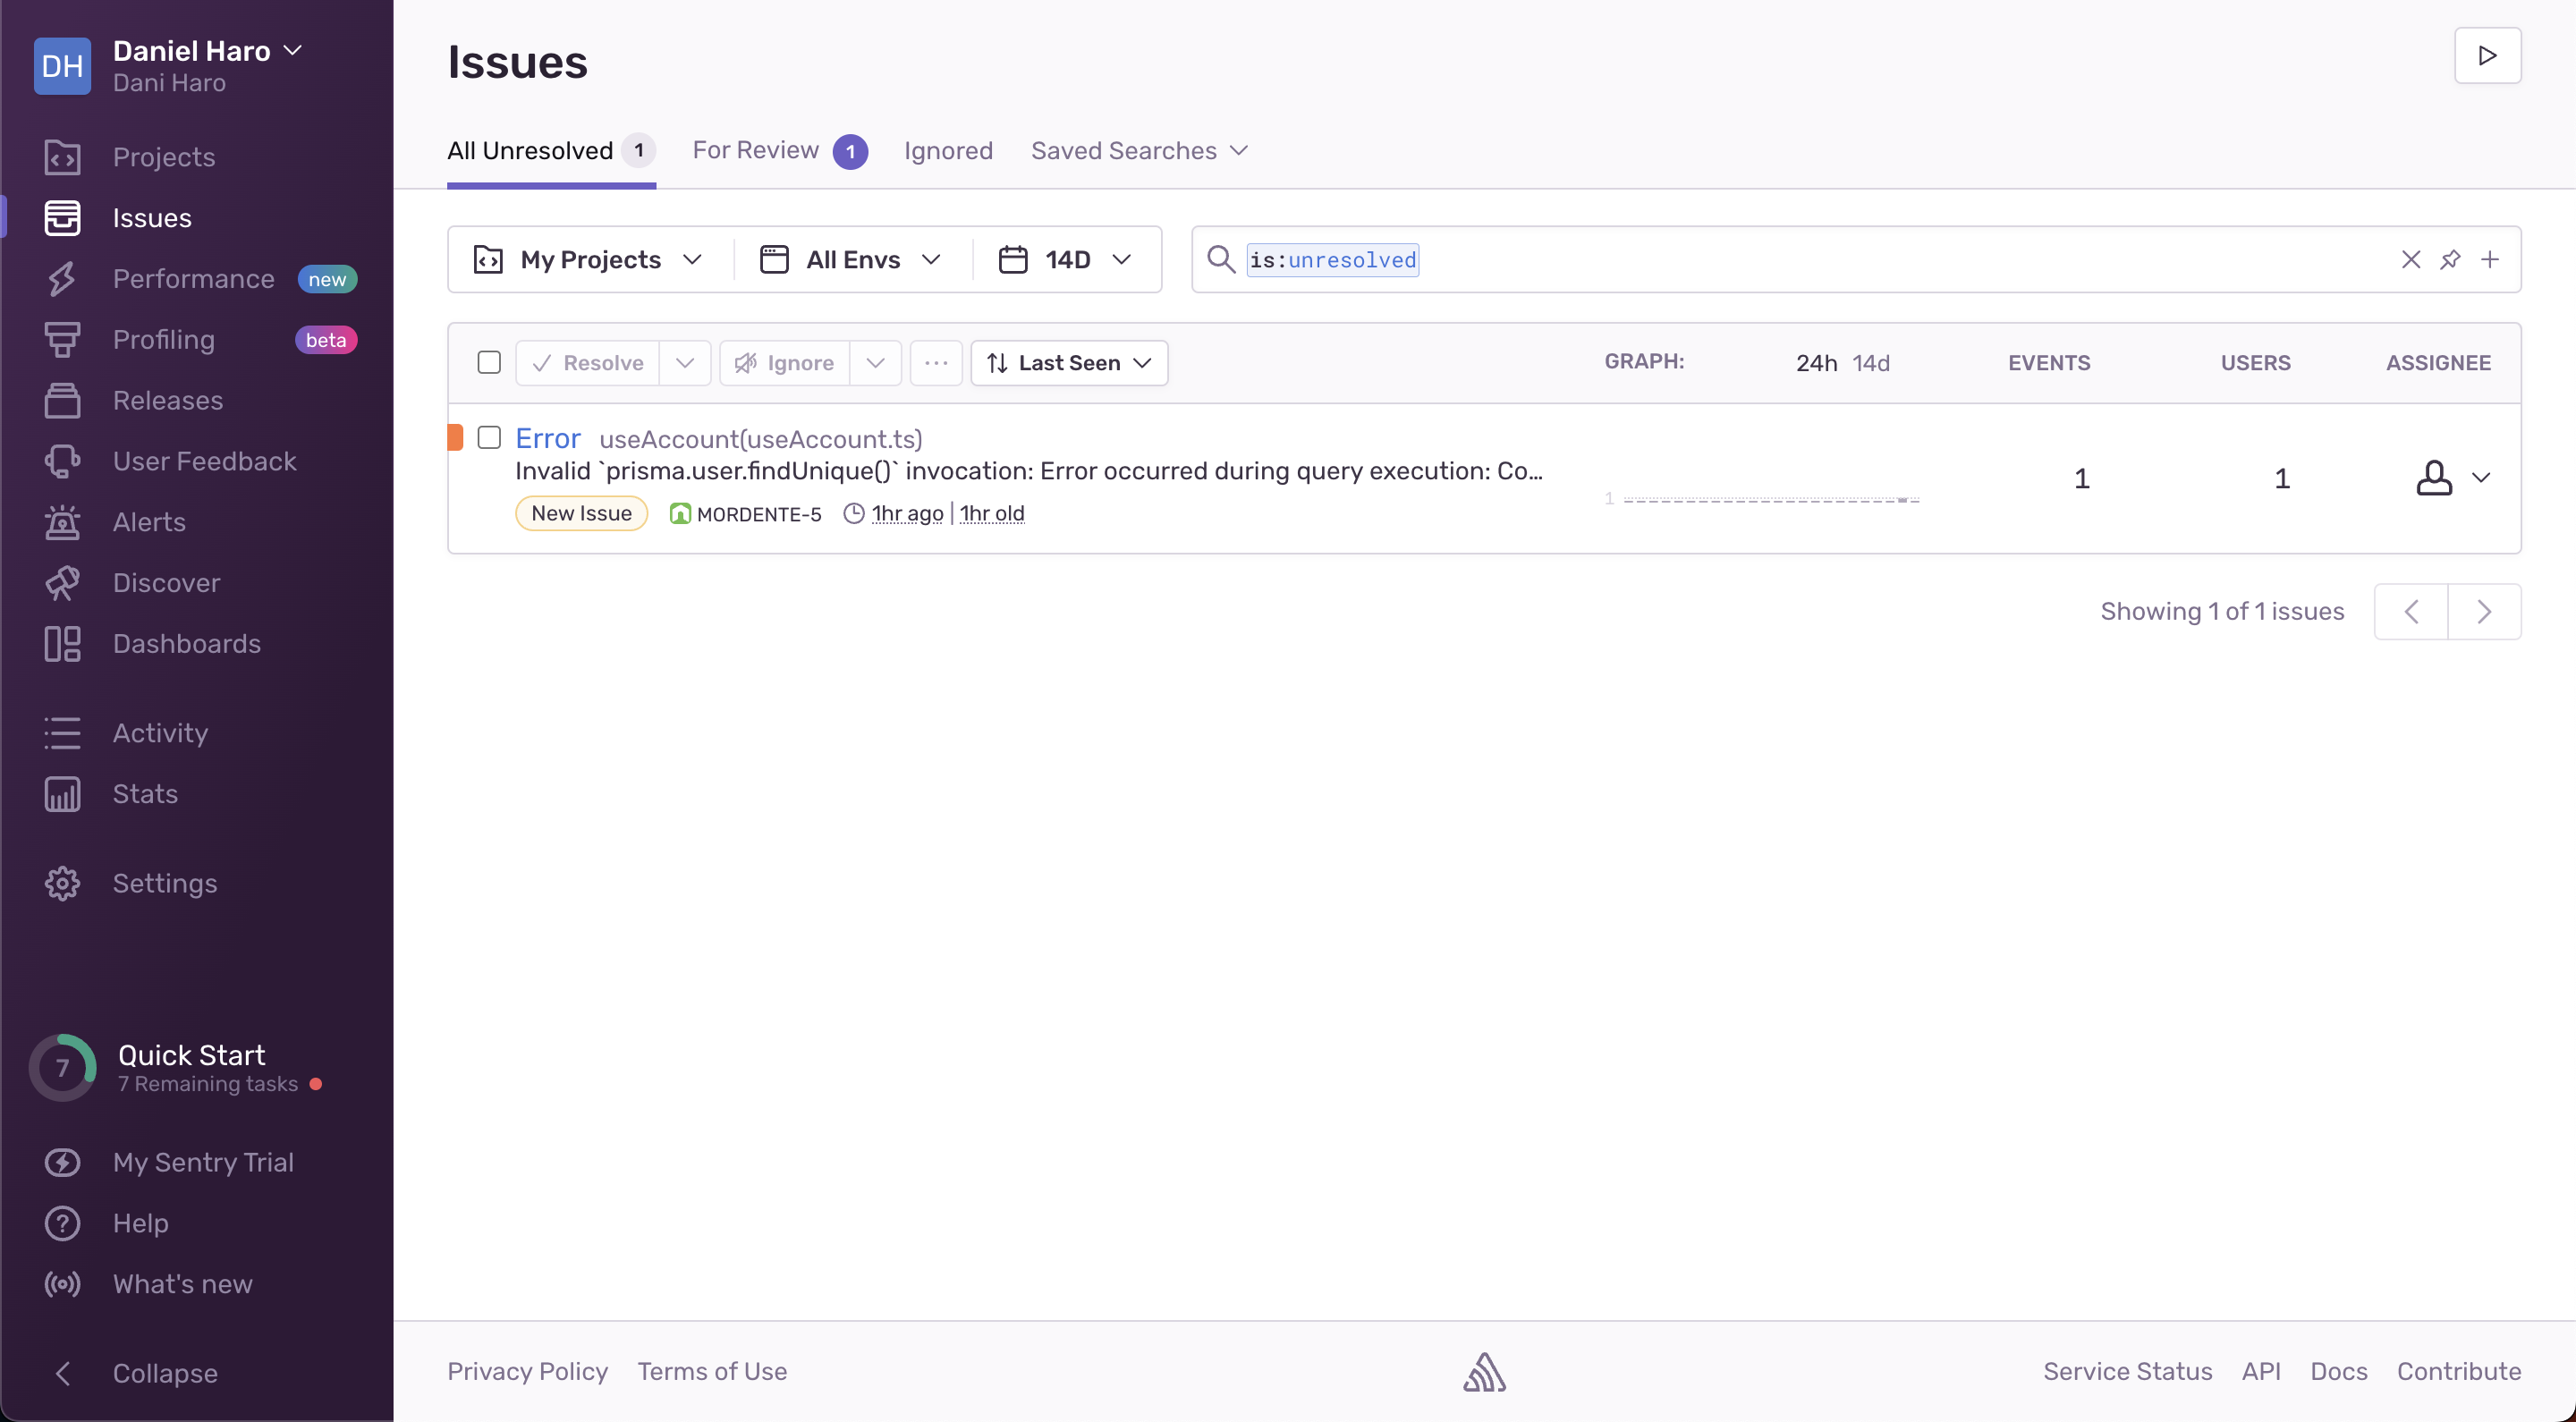
\includegraphics[width=\textwidth]{imagenes/pruebas/sentry_error_uid.png}
\caption{Lista de errores registrados en Sentry}
\label{fig:sentryListaErrores}
\end{figure}

\begin{figure}[h]
\centering
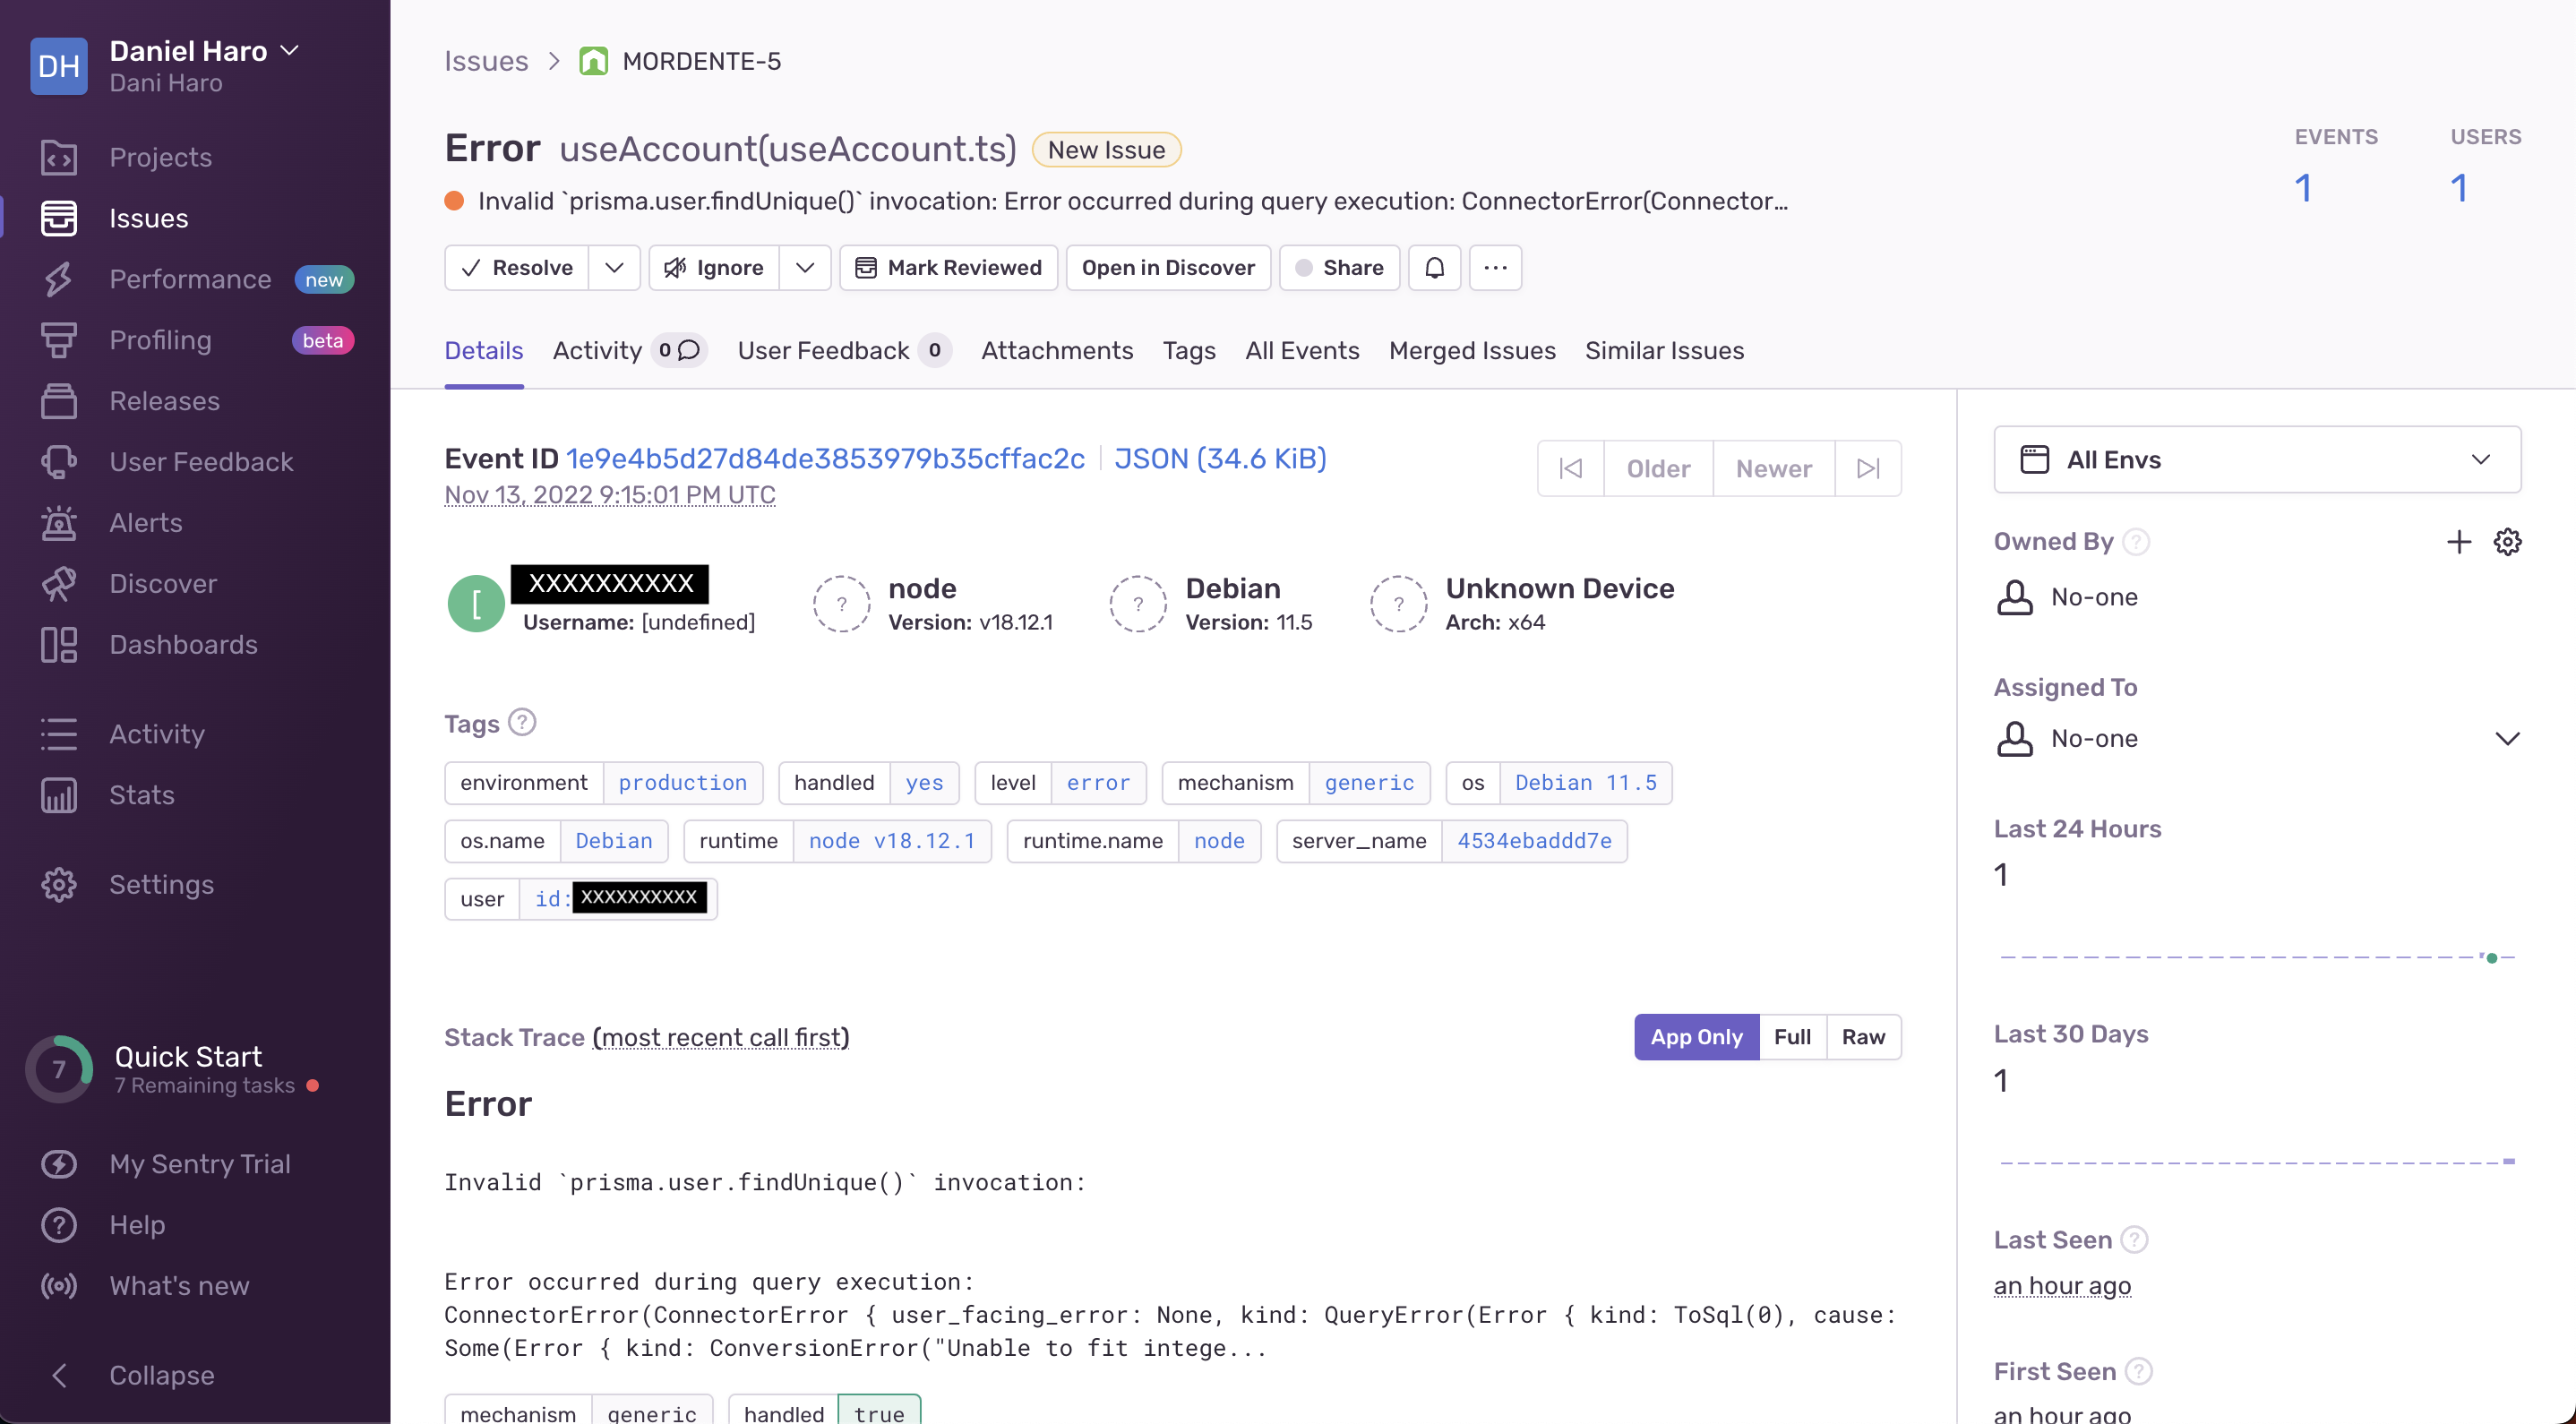
\includegraphics[width=\textwidth]{imagenes/pruebas/sentry_detalle_error_uid.png}
\caption{Detalle del error generado por desbordamiento del ID de Telegram}
\label{fig:sentryDetalleError}
\end{figure}

\subsection{Peticiones}

Una de las peticiones más populares ha sido la de incorporar la funcionalidad de \textbf{calendario} ya que la alternativa que se ha analizado en la sección \ref{subsection:glissandoo} no la implementa. Dado que requiere de más esfuerzo para su implementación, se ha programado como trabajo futuro.


\section{Demostración en vídeo}

Se puede visualizar el funcionamiento del bot en el vídeo disponible el siguiente enlace:

\url{https://mordente.es/video/demo}

